%=============================================================================
% paper.tex
% CNN-Based Modulation Format Identification for Optical Performance Monitoring
%
% IEEE conference format (IEEEtran). Compile with:
%     python paper/make_macros.py        <- regenerates every number
%     pdflatex paper.tex
%     bibtex   paper
%     pdflatex paper.tex
%     pdflatex paper.tex
%
% Every numerical result in the text is a macro defined in
% results_macros.tex, which is generated directly from the experiment JSON.
% That means the prose can never drift out of step with the tables.
%=============================================================================
\documentclass[conference]{IEEEtran}
\IEEEoverridecommandlockouts

\usepackage{cite}
\usepackage{amsmath,amssymb}
\usepackage{graphicx}
\usepackage{booktabs}
\usepackage{multirow}
\usepackage{url}
\usepackage[caption=false,font=footnotesize]{subfig}

\graphicspath{{../figures/}}

% ---- auto-generated numbers -------------------------------------------------
% results_macros.tex -- AUTO-GENERATED by paper/make_macros.py
% Do not edit by hand: re-run the script instead.
% Every number in the manuscript comes from here, so the text can
% never disagree with the experiments.

\newcommand{\AblBestAcc}{98.37}
\newcommand{\AblBestBlocks}{3}
\newcommand{\AblBestCh}{4}
\newcommand{\AblBigAcc}{98.28}
\newcommand{\AblBigParams}{617,573}
\newcommand{\AblFourBlockAcc}{98.22}
\newcommand{\AblMacRatio}{49}
\newcommand{\AblMax}{98.37}
\newcommand{\AblMin}{97.11}
\newcommand{\AblParamRatio}{9.2}
\newcommand{\AblSpread}{1.26}
\newcommand{\AblThreeBlockAcc}{98.15}
\newcommand{\AblTinyAcc}{98.37}
\newcommand{\AblTinyCh}{4}
\newcommand{\AblTinyMacs}{0.80}
\newcommand{\AblTinyParams}{67,457}
\newcommand{\AblTwoBlockAcc}{97.94}
\newcommand{\BudgetCNNCD}{50}
\newcommand{\BudgetCNNFoff}{50}
\newcommand{\BudgetCNNGain}{2.5}
\newcommand{\BudgetCNNLw}{2000}
\newcommand{\BudgetCNNSkew}{14}
\newcommand{\BudgetSVMCD}{90}
\newcommand{\BudgetSVMFoff}{50}
\newcommand{\BudgetSVMGain}{0.6}
\newcommand{\BudgetSVMLw}{2000}
\newcommand{\BudgetSVMSkew}{4}
\newcommand{\CNNGenAcc}{97.45}
\newcommand{\CNNGenDrop}{1.27}
\newcommand{\CNNGenStd}{0.16}
\newcommand{\CNNOSNRNinetyFive}{7}
\newcommand{\CNNOSNRNinetyNine}{10}
\newcommand{\CNNacc}{98.73}
\newcommand{\CNNaccHigh}{100.00}
\newcommand{\CNNaccLow}{95.57}
\newcommand{\CNNmacs}{10.3}
\newcommand{\CNNparams}{285,941}
\newcommand{\CNNstd}{0.12}
\newcommand{\ChanceLevel}{20}
\newcommand{\ConfCNNAcc90}{96.77}
\newcommand{\ConfCNNCov90}{86.9}
\newcommand{\ConfCNNsevAcc}{89.78}
\newcommand{\ConfCNNsevAuroc}{0.947}
\newcommand{\ConfCNNsevConf}{95.67}
\newcommand{\ConfCNNsevOver}{5.89}
\newcommand{\ConfMLPAcc90}{99.59}
\newcommand{\ConfMLPCov90}{63.7}
\newcommand{\ConfMLPsevAcc}{85.46}
\newcommand{\ConfMLPsevAuroc}{0.925}
\newcommand{\ConfMLPsevConf}{83.78}
\newcommand{\ConfMLPsevOver}{-1.68}
\newcommand{\ConfSVMAcc90}{100.00}
\newcommand{\ConfSVMCov90}{0.2}
\newcommand{\ConfSVMmodCov90}{5.3}
\newcommand{\ConfSVMmodSevAcc}{76.15}
\newcommand{\ConfSVMmodSevOver}{-20.69}
\newcommand{\ConfSVMsevAcc}{22.41}
\newcommand{\ConfSVMsevAuroc}{0.949}
\newcommand{\ConfSVMsevConf}{42.95}
\newcommand{\ConfSVMsevOver}{20.54}
\newcommand{\CovRatio}{447}
\newcommand{\FeatBest}{93.41}
\newcommand{\FeatSpread}{1.83}
\newcommand{\FeatWorst}{91.58}
\newcommand{\FormatList}{QPSK, 8-QAM, 16-QAM, 32-QAM, 64-QAM}
\newcommand{\IQCNNOSNRNinetyFive}{--}
\newcommand{\IQCNNOSNRNinetyNine}{--}
\newcommand{\IQCNNacc}{86.56}
\newcommand{\IQCNNaccHigh}{91.68}
\newcommand{\IQCNNaccLow}{77.25}
\newcommand{\IQCNNmacs}{4.4}
\newcommand{\IQCNNparams}{27,781}
\newcommand{\IQCNNstd}{4.64}
\newcommand{\ImgSize}{64}
\newcommand{\KNNOSNRNinetyFive}{15}
\newcommand{\KNNOSNRNinetyNine}{18}
\newcommand{\KNNacc}{91.58}
\newcommand{\KNNaccHigh}{99.95}
\newcommand{\KNNaccLow}{80.88}
\newcommand{\KNNstd}{0.08}
\newcommand{\MLPGenAcc}{92.82}
\newcommand{\MLPGenDrop}{0.25}
\newcommand{\MLPGenStd}{0.19}
\newcommand{\MLPOSNRNinetyFive}{14}
\newcommand{\MLPOSNRNinetyNine}{18}
\newcommand{\MLPacc}{93.08}
\newcommand{\MLPaccHigh}{99.98}
\newcommand{\MLPaccLow}{82.23}
\newcommand{\MLPmacs}{0.010}
\newcommand{\MLPparams}{11,013}
\newcommand{\MLPstd}{0.10}
\newcommand{\NumFormats}{5}
\newcommand{\NumImages}{63,000}
\newcommand{\NumOSNR}{21}
\newcommand{\NumSeeds}{3}
\newcommand{\NumSymbols}{4096}
\newcommand{\OSNRMargin}{7}
\newcommand{\OSNRmax}{25}
\newcommand{\OSNRmin}{5}
\newcommand{\RepGain}{5.32}
\newcommand{\RepRatio}{2.9}
\newcommand{\RobCNNDrop}{8.13}
\newcommand{\RobIdealIdealCNN}{97.92}
\newcommand{\RobIdealIdealSVM}{93.02}
\newcommand{\RobIdealRealCNN}{98.11}
\newcommand{\RobIdealSevereCNN}{89.78}
\newcommand{\RobIdealSevereSVM}{21.84}
\newcommand{\RobRealRealCNN}{98.27}
\newcommand{\RobRealSevereCNN}{91.17}
\newcommand{\RobRealSevereSVM}{71.98}
\newcommand{\RobSVMDrop}{71.18}
\newcommand{\SVMGenAcc}{93.05}
\newcommand{\SVMGenDrop}{0.36}
\newcommand{\SVMGenStd}{0.04}
\newcommand{\SVMOSNRNinetyFive}{14}
\newcommand{\SVMOSNRNinetyNine}{18}
\newcommand{\SVMacc}{93.41}
\newcommand{\SVMaccHigh}{99.94}
\newcommand{\SVMaccLow}{83.05}
\newcommand{\SVMstd}{0.10}
\newcommand{\SymEnough}{512}
\newcommand{\SymEnoughAcc}{94.08}
\newcommand{\SymMax}{4096}
\newcommand{\SymMaxAcc}{97.84}
\newcommand{\SymMin}{128}
\newcommand{\SymMinAcc}{90.31}
\newcommand{\SymbolRate}{32}
\newcommand{\TolCNNcdHi}{54.89}
\newcommand{\TolCNNgainHi}{95.48}
\newcommand{\TolCNNskewHi}{96.35}
\newcommand{\TolSVMcdHi}{80.14}
\newcommand{\TolSVMgainHi}{20.35}
\newcommand{\TolSVMgainLo}{93.11}
\newcommand{\TolSVMskewHi}{20.10}
\newcommand{\TolSVMskewLo}{93.11}


\begin{document}

\title{Input Representation Dominates Model Choice in\\
Machine-Learning Modulation Format Identification}

\author{\IEEEauthorblockN{Nitesh Kumar Yadav}
\IEEEauthorblockA{\textit{Department of Electronics and Communication Engineering}\\
\textit{[Institution]}\\
Delhi, India \\
niteshkumar88449@gmail.com}
}

\maketitle

%=============================================================================
\begin{abstract}
Modulation format identification (MFI) lets a coherent optical receiver
determine the incoming format without a control channel, and is a core
function of optical performance monitoring in elastic optical networks.
Convolutional neural networks (CNNs) applied to constellation diagrams are
known to outperform classical feature-based classifiers, but the reported
comparisons change two variables at once: the learning algorithm becomes
deep, \emph{and} the input becomes a two-dimensional image. It is therefore
unclear whether the reported gains come from the model or from the
representation. We disentangle the two on a common simulated benchmark of
\NumImages{} constellation captures spanning \NumFormats{} formats
(\FormatList) and OSNR from \OSNRmin{} to \OSNRmax~dB, generated with a
channel model that includes laser phase noise, residual frequency offset,
I/Q imbalance and residual chromatic dispersion in addition to ASE noise. We
evaluate five classifiers over three input representations: raw I/Q samples,
a $\ImgSize\times\ImgSize$ constellation density image, and $15$ higher-order
statistical features. Holding the representation fixed and varying the
algorithm across a multilayer perceptron, a support vector machine and a
$k$-nearest-neighbour classifier changes accuracy by only \FeatSpread{}
percentage points; holding the algorithm class fixed and changing the
representation from features to the density image changes it by \RepGain{}
points. The image-based CNN attains \CNNacc$\pm$\CNNstd\% overall and reaches
$95\%$ accuracy \OSNRMargin~dB earlier in OSNR than the best feature-based
model. The gap widens sharply under distribution shift: trained on an
AWGN-only channel and tested on a severely impaired one, the CNN retains
\RobIdealSevereCNN\% while the feature-based classifier falls to
\RobIdealSevereSVM\%, essentially the \ChanceLevel\% chance level. We further
show that the learned model interpolates to OSNR values withheld from
training, that a \SymEnough-symbol capture processed as an image outperforms a
\SymMax-symbol capture reduced to features, and that accuracy is insensitive
to model capacity across a \AblParamRatio$\times$ range of parameter counts.
The results indicate that, for this task, effort is better spent on the input
representation than on model capacity --- and that reporting only
matched-channel accuracy can conceal a complete loss of function under
realistic deployment conditions.
\end{abstract}

\begin{IEEEkeywords}
Modulation format identification, optical performance monitoring,
convolutional neural network, constellation diagram, coherent detection,
machine learning.
\end{IEEEkeywords}

%=============================================================================
\section{Introduction}

Elastic optical networks adapt the modulation format of each lightpath to the
conditions of the link, using dense formats such as 64-QAM on short, clean
routes and robust formats such as QPSK on long, noisy ones. Before a coherent
receiver can demodulate anything it must know which format has arrived,
because the decision rules differ for each. Conventionally this is negotiated
through a control channel. \emph{Modulation format identification} (MFI)
removes that dependency by inferring the format from the received signal
itself, enabling faster reconfiguration and more autonomous operation, and it
is a standard component of optical performance monitoring
(OPM)~\cite{khan2019perspective}.

Classical MFI relies on hand-crafted statistics of the received samples,
most commonly higher-order cumulants, which have the useful property that the
contribution of Gaussian noise cancels at fourth order and
above~\cite{swami2000cumulants,dobre2007survey}. These features are fed to a
conventional classifier such as a support vector machine (SVM) or a
$k$-nearest-neighbour ($k$-NN) rule. More recently, deep learning has been
applied directly to the constellation diagram, treating MFI as an image
classification problem, with reported gains over the classical
pipeline~\cite{wang2017analyzer,khan2016deep,oshea2016radio}.

The comparison underlying these gains, however, varies two factors at once. A
CNN operating on a constellation image differs from an SVM operating on
cumulants both in the model, which is deep and learned rather than shallow and
kernel-based, and in the input, which is a two-dimensional density map rather
than a short vector of summary statistics. In the wireless AMC literature this
confound has been addressed by holding the classifier fixed and varying the
representation~\cite{ge2021accuracy}; in the optical domain, where the
impairments differ substantially, we are not aware of an equivalent controlled
comparison.

This paper separates them by holding one factor fixed while varying the other.
We find that the representation dominates: three learning algorithms of very
different type, given identical features, span \FeatSpread{} percentage
points, whereas changing the input to a density image gains \RepGain{} points.
The difference is larger still under channel mismatch, where the feature-based
classifier loses essentially all discriminative ability while the CNN degrades
gradually. Our contributions are:

\begin{enumerate}
\item A controlled comparison of five classifiers across three input
      representations on identical signals, which separates the effect of the
      \emph{model} from the effect of the \emph{representation}. In
      particular we add a multilayer perceptron (MLP) on the same $15$
      features given to the SVM and $k$-NN, so that ``deep model'' and
      ``image input'' are varied independently.
\item A channel model that goes beyond additive white Gaussian noise (AWGN)
      to include laser phase noise with block-average carrier phase recovery,
      residual frequency offset, receiver I/Q gain imbalance and phase skew,
      and residual chromatic dispersion.
\item Evidence that the learned model generalises to OSNR levels withheld
      from training, addressing the concern that such models merely memorise
      the appearance of each noise level.
\item An accuracy--complexity study, together with the shortest capture length
      that still supports reliable identification. Both quantities constrain a
      monitoring receiver with a limited compute and memory budget, and
      neither is commonly reported.
\item A cross-channel robustness study quantifying the loss incurred when a
      model trained on one channel model is applied to a more heavily impaired
      one. We find this loss to differ by an order of magnitude between the
      two representations.
\end{enumerate}

All code, data-generation scripts and trained models are released, and every
number reported here is reproducible from a fixed random seed.

%=============================================================================
\section{Related Work}

Automatic modulation classification has a long history in wireless
communications, where cumulant-based decision trees and feature classifiers
were established well before deep learning~\cite{swami2000cumulants,
dobre2007survey}. O'Shea \emph{et al.}~\cite{oshea2016radio} showed that
convolutional networks operating on raw sampled waveforms could match or
exceed expert-feature approaches for radio signals.

In the optical domain, Khan \emph{et al.}~\cite{khan2016deep} applied deep
neural networks to asynchronous amplitude histograms for joint OSNR
monitoring and format identification, and Wang \emph{et al.}
\cite{wang2017analyzer} introduced the ``intelligent constellation diagram
analyser'', in which a CNN classifies constellation images and simultaneously
estimates OSNR. A broad survey of machine learning for optical communications
is given in~\cite{khan2019perspective}.

The question of input representation has been addressed directly in the
\emph{wireless} AMC literature. Ge \emph{et al.}~\cite{ge2021accuracy} compare
five representations --- higher-order cumulants, fuzzy $c$-means features,
grid-like constellation diagrams, cumulative distribution functions and raw
I/Q --- while holding the classifier fixed, and report that cumulants, raw I/Q
and grid constellations perform comparably under a Gaussian channel, whereas
cumulant performance degrades markedly under non-Gaussian conditions. A recent
survey~\cite{amcsurvey2025} organises the DL-AMC literature explicitly by data
representation. Our study is complementary in three respects: it addresses the
optical channel, in which OSNR and transceiver impairments rather than
multipath dominate; it varies the algorithm as well as the representation, so
that both directions of the comparison are controlled; and it reaches a
different conclusion for the matched-channel case, where we find the density
image to be clearly superior rather than comparable.

Within optical MFI, image-derived features have been used with conventional
classifiers: Huang \emph{et al.}~\cite{huang2022svm} extract fractal-dimension
and grey-level co-occurrence features from constellation diagrams and classify
them with an SVM, reporting 100\% accuracy above 10~dB OSNR for seven formats.
That work varies the representation but not the classifier, and evaluates
under a single channel condition.

The cross-channel evaluation of Section~\ref{sec:robustness}, in which a model
trained under one impairment profile is tested under another, appears to be
less commonly reported for optical MFI; where generalisation is studied it is
typically across OSNR within a fixed impairment model.

%=============================================================================
\section{System Model and Dataset}

\subsection{Transmitter}

We consider single-polarisation coherent transmission at
$R_s = \SymbolRate$~GBaud. Symbols are drawn uniformly from one of
\NumFormats{} constellations: QPSK, star 8-QAM, square 16-QAM, cross 32-QAM
and square 64-QAM. Two of these are deliberately non-square, so that a
classifier cannot succeed merely by distinguishing square grids of different
densities. Every constellation is normalised to unit average power,
$\mathbb{E}[|s|^2]=1$. This normalisation is essential: without it the
formats would differ in received power and any classifier could identify them
trivially, whereas a real receiver applies automatic gain control and always
delivers a fixed power.

\subsection{Channel and receiver impairments}

The received sample sequence is generated as
\begin{equation}
r[k] = \mathcal{G}\!\left\{ \mathcal{I}\!\left[ \mathcal{P}\!\left(
       \mathcal{D}\{s[k]\} \right) \right] \right\} + n[k],
\end{equation}
where $\mathcal{D}$ applies residual chromatic dispersion, $\mathcal{P}$
applies laser phase noise and frequency offset followed by carrier phase
recovery, $\mathcal{I}$ applies receiver I/Q imbalance, $\mathcal{G}$ is
automatic gain control, and $n[k]$ is circularly symmetric AWGN modelling
amplified spontaneous emission.

\textbf{Residual chromatic dispersion} is modelled as an all-pass filter with
quadratic phase, $H(\omega)=\exp\!\left(j\frac{\beta_2 L}{2}\omega^2\right)$
with $\beta_2 L = -\frac{\lambda^2}{2\pi c}D_{\mathrm{tot}}$, retaining the
inter-symbol interference that survives electronic compensation.

\textbf{Laser phase noise} is a Wiener process with per-symbol variance
$2\pi\,\Delta\nu\,T_s$. A frequency offset $\Delta f$ contributes an
additional linear phase ramp. Both are then passed through a block-average
carrier phase estimator of length $64$ symbols, which removes the slowly
varying component of each. What survives is the phase variation \emph{within}
one estimation block. This ordering matters: applying a frequency offset
after phase recovery, as is sometimes done, leaves it uncorrected and smears
each constellation point into an arc, which does not represent the output of
a functioning receiver.

\textbf{I/Q imbalance} applies a gain mismatch between the in-phase and
quadrature arms together with a departure from the ideal $90^\circ$ hybrid
phase, which skews the constellation rather than blurring it.

Three impairment profiles are defined --- \textsc{ideal} (AWGN only),
\textsc{realistic}, and \textsc{severe} --- and are used in
Section~\ref{sec:robustness}. Unless stated otherwise, results use
\textsc{realistic}.

\subsection{OSNR to SNR conversion}

OSNR is an optical quantity measured in a fixed $0.1$~nm ($12.5$~GHz)
reference bandwidth across both polarisations, whereas the electrical SNR
seen by the receiver follows
\begin{equation}
\mathrm{SNR} = \mathrm{OSNR}\cdot\frac{2B_{\mathrm{ref}}}{p R_s},
\end{equation}
which for our parameters gives
$\mathrm{SNR}_{\mathrm{dB}}=\mathrm{OSNR}_{\mathrm{dB}}-1.07$~dB. Reporting
against OSNR without this conversion overstates the electrical SNR by roughly
$1$~dB.

\subsection{Simulator validation}

Before any learning, the simulator is validated against theory. For a
noiseless unit-power constellation the normalised fourth-order cumulant
$|C_{40}|/C_{21}^2$ is an exact finite sum over the constellation points. The
simulator reproduces these values for all \NumFormats{} formats to within
$0.004$, and the three square formats additionally match the standard
published constants ($1.0000$, $0.6800$, $0.6191$). We compute the reference
values analytically rather than quoting them from the literature because
8-QAM and 32-QAM each have several standard variants with different
cumulants.

\subsection{Dataset}

For each of the \NumFormats{} formats and each of the \NumOSNR{} OSNR values
from \OSNRmin{} to \OSNRmax~dB in $1$~dB steps we generate independent
captures of \NumSymbols{} symbols, giving \NumImages{} examples in total.
Each capture is converted into three representations:

\begin{itemize}
\item \textbf{Raw I/Q}: the first $512$ complex samples as a $2\times512$
      real array. No human pre-processing.
\item \textbf{Constellation image}: a $\ImgSize\times\ImgSize$
      two-dimensional histogram of the samples over
      $I,Q\in[-2.5,2.5]$, with logarithmic intensity scaling. The same
      spatial range is used for every format, so the zoom level carries no
      class information. Logarithmic scaling preserves the sparse outer
      constellation points, which a linear scale would quantise to zero.
\item \textbf{Statistical features}: $15$ numbers comprising seven normalised
      higher-order cumulants ($|C_{20}|$, $|C_{40}|$, $|C_{41}|$, $|C_{42}|$,
      $|C_{60}|$, $|C_{61}|$, $|C_{63}|$) and eight amplitude- and
      phase-distribution statistics.
\end{itemize}

Crucially, all three representations are derived from the \emph{same}
realisation, so any performance difference is attributable to the
representation and not to differing data.

Data are split $70/15/15$ into training, validation and test sets,
stratified jointly on (format, OSNR) so that each of the
$\NumFormats\times\NumOSNR$ cells is divided in the same proportion. The test
set is used exactly once.

\begin{figure}[t]
\centering
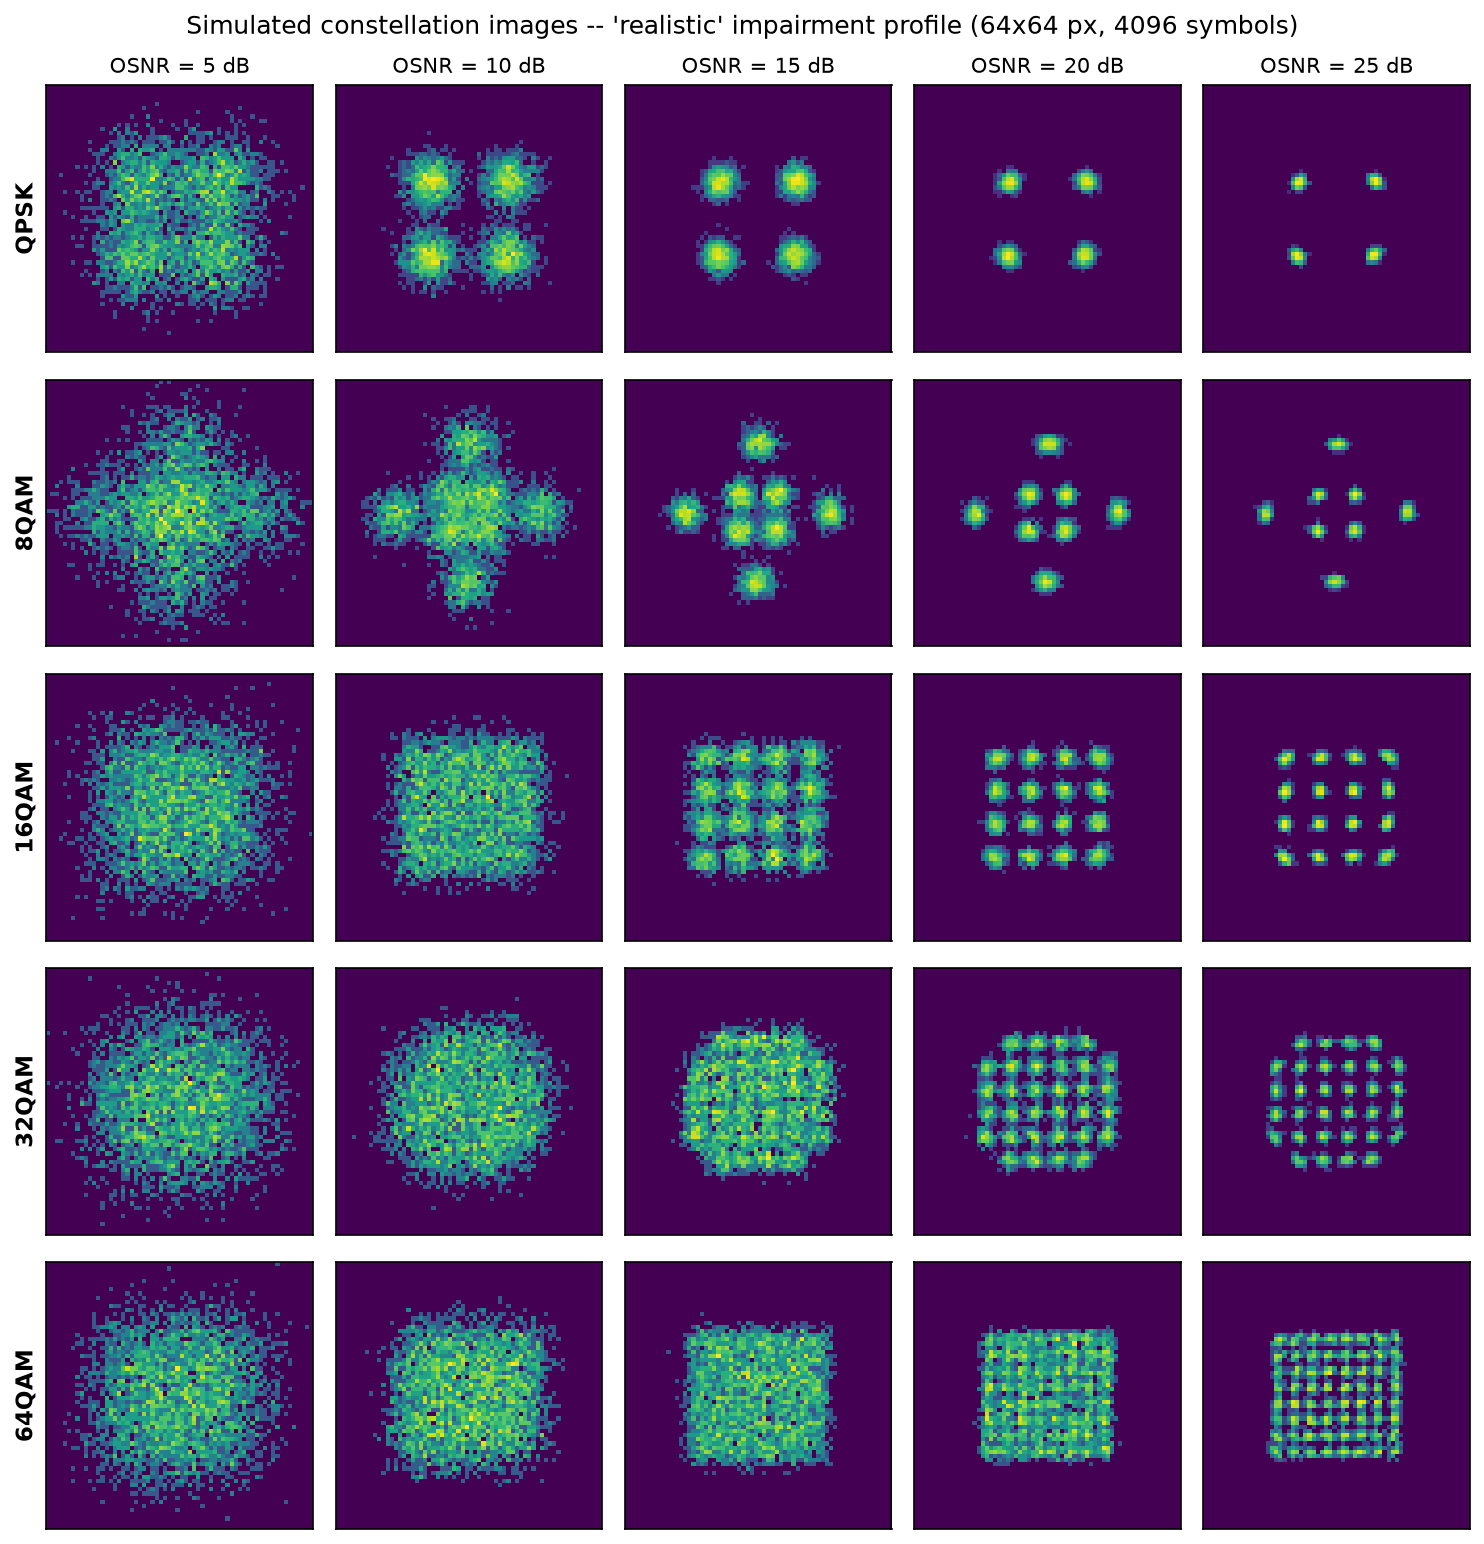
\includegraphics[width=\columnwidth]{sample_constellations.png}
\caption{Example constellation images under the \textsc{realistic}
impairment profile. Denser constellations require substantially higher OSNR
to remain resolvable, which is the physical mechanism behind the
accuracy--OSNR curves of Fig.~\ref{fig:acc_osnr}.}
\label{fig:samples}
\end{figure}

%=============================================================================
\section{Classifiers and Representations}

We evaluate five classifiers, chosen so that the model and the representation
can be varied independently (Table~\ref{tab:main}).

\subsection{Image representation: 2-D CNN}
Three convolutional blocks (\texttt{Conv}$3\times3$--\texttt{BN}--%
\texttt{ReLU}--\texttt{MaxPool}$2$) with $16$, $32$ and $64$ channels, then
dropout and two fully connected layers. After three pooling stages one
feature-map element covers roughly a $30\times30$ region of the input, which
matches the scale of the constellation structure to be recognised. Features
are flattened rather than globally average-pooled, because the geometric
\emph{arrangement} of clusters in the I/Q plane is precisely the
discriminative information; discarding position would discard the signal.

\subsection{Raw I/Q representation: 1-D CNN}
Three 1-D convolutional blocks (kernels $7$, $5$, $3$; $32$, $64$, $64$
channels) followed by global average pooling. Here pooling over position
\emph{is} appropriate, because the symbol stream is stationary and absolute
position within the capture carries no information. This model represents the
zero-pre-processing extreme.

\subsection{Feature representation: MLP, SVM, $k$-NN}
The MLP has hidden layers of $128$ and $64$ units with batch normalisation
and dropout. The SVM uses an RBF kernel with $C=10$; the $k$-NN uses $k=5$.
All three are preceded by standardisation whose statistics are estimated on
the training partition only, to avoid leakage. The MLP is the critical
control: it is a trained deep network that sees only the hand-crafted
features, so comparing it against the CNN isolates the representation, while
comparing it against the SVM and $k$-NN isolates the algorithm.

Networks are trained with Adam ($\eta=10^{-3}$, weight decay $10^{-4}$),
batch size $128$, learning-rate halving on plateau, and early stopping on
validation accuracy. All experiments are repeated over \NumSeeds{} random
seeds and reported as mean $\pm$ standard deviation.

%=============================================================================
\section{Results}

\subsection{Overall comparison}

Table~\ref{tab:main} reports overall test accuracy. The image-based CNN
attains \CNNacc$\pm$\CNNstd\%. The three feature-based classifiers attain
\MLPacc\%, \SVMacc\% and \KNNacc\% respectively, and the raw-I/Q 1-D CNN
attains \IQCNNacc\%.

\begin{table}[t]
\caption{Overall test accuracy by input representation
(mean $\pm$ s.d. over \NumSeeds{} seeds).}
\label{tab:main}
\centering
\begin{tabular}{llrr}
\toprule
Model & Input representation & Accuracy (\%) & Params \\
\midrule
CNN      & $\ImgSize\times\ImgSize$ image & \CNNacc\ $\pm$ \CNNstd   & \CNNparams \\
IQ-CNN   & $512$ raw I/Q samples          & \IQCNNacc\ $\pm$ \IQCNNstd & \IQCNNparams \\
MLP      & $15$ features                  & \MLPacc\ $\pm$ \MLPstd   & \MLPparams \\
SVM      & $15$ features                  & \SVMacc\ $\pm$ \SVMstd   & --- \\
$k$-NN   & $15$ features                  & \KNNacc\ $\pm$ \KNNstd   & --- \\
\bottomrule
\end{tabular}
\end{table}

\subsection{Representation versus algorithm}

Table~\ref{tab:main} and Fig.~\ref{fig:representation} report the main
comparison. Three learning algorithms of very different type (a trained deep
network, a kernel method, and a non-parametric nearest-neighbour rule)
operating on identical inputs span only \FeatSpread{} percentage points.
Replacing the input with the constellation density image, while keeping the
model a convolutional network of comparable scale, gains \RepGain{} points
over the best of the three.

The choice of algorithm therefore accounts for \FeatSpread{} points of
variation, and the choice of representation for \RepGain{} points, a ratio of
approximately \RepRatio. We take this as evidence that the representation is
the dominant design variable for this task.

The raw-I/Q model is both the weakest and the least stable, with a standard
deviation across seeds of \IQCNNstd{} points against $\leq \CNNstd$ for the
other four models. Its exact position is therefore treated as uncertain, and
only its ordering (worst in all \NumSeeds{} runs) is relied upon below.

That the raw-I/Q representation performs worst, despite discarding no
information, can be explained by the statistics of the signal. The
transmitted symbols are independent and identically distributed, so temporal
order carries little information about the format, whereas a 1-D convolution
is structured to exploit order. The network must therefore estimate a
distribution from a sequence. A 2-D histogram is itself a density estimate,
so binning performs part of that estimation before training begins. We
attribute the observed gain to this effect rather than to model capacity.

\begin{figure}[t]
\centering
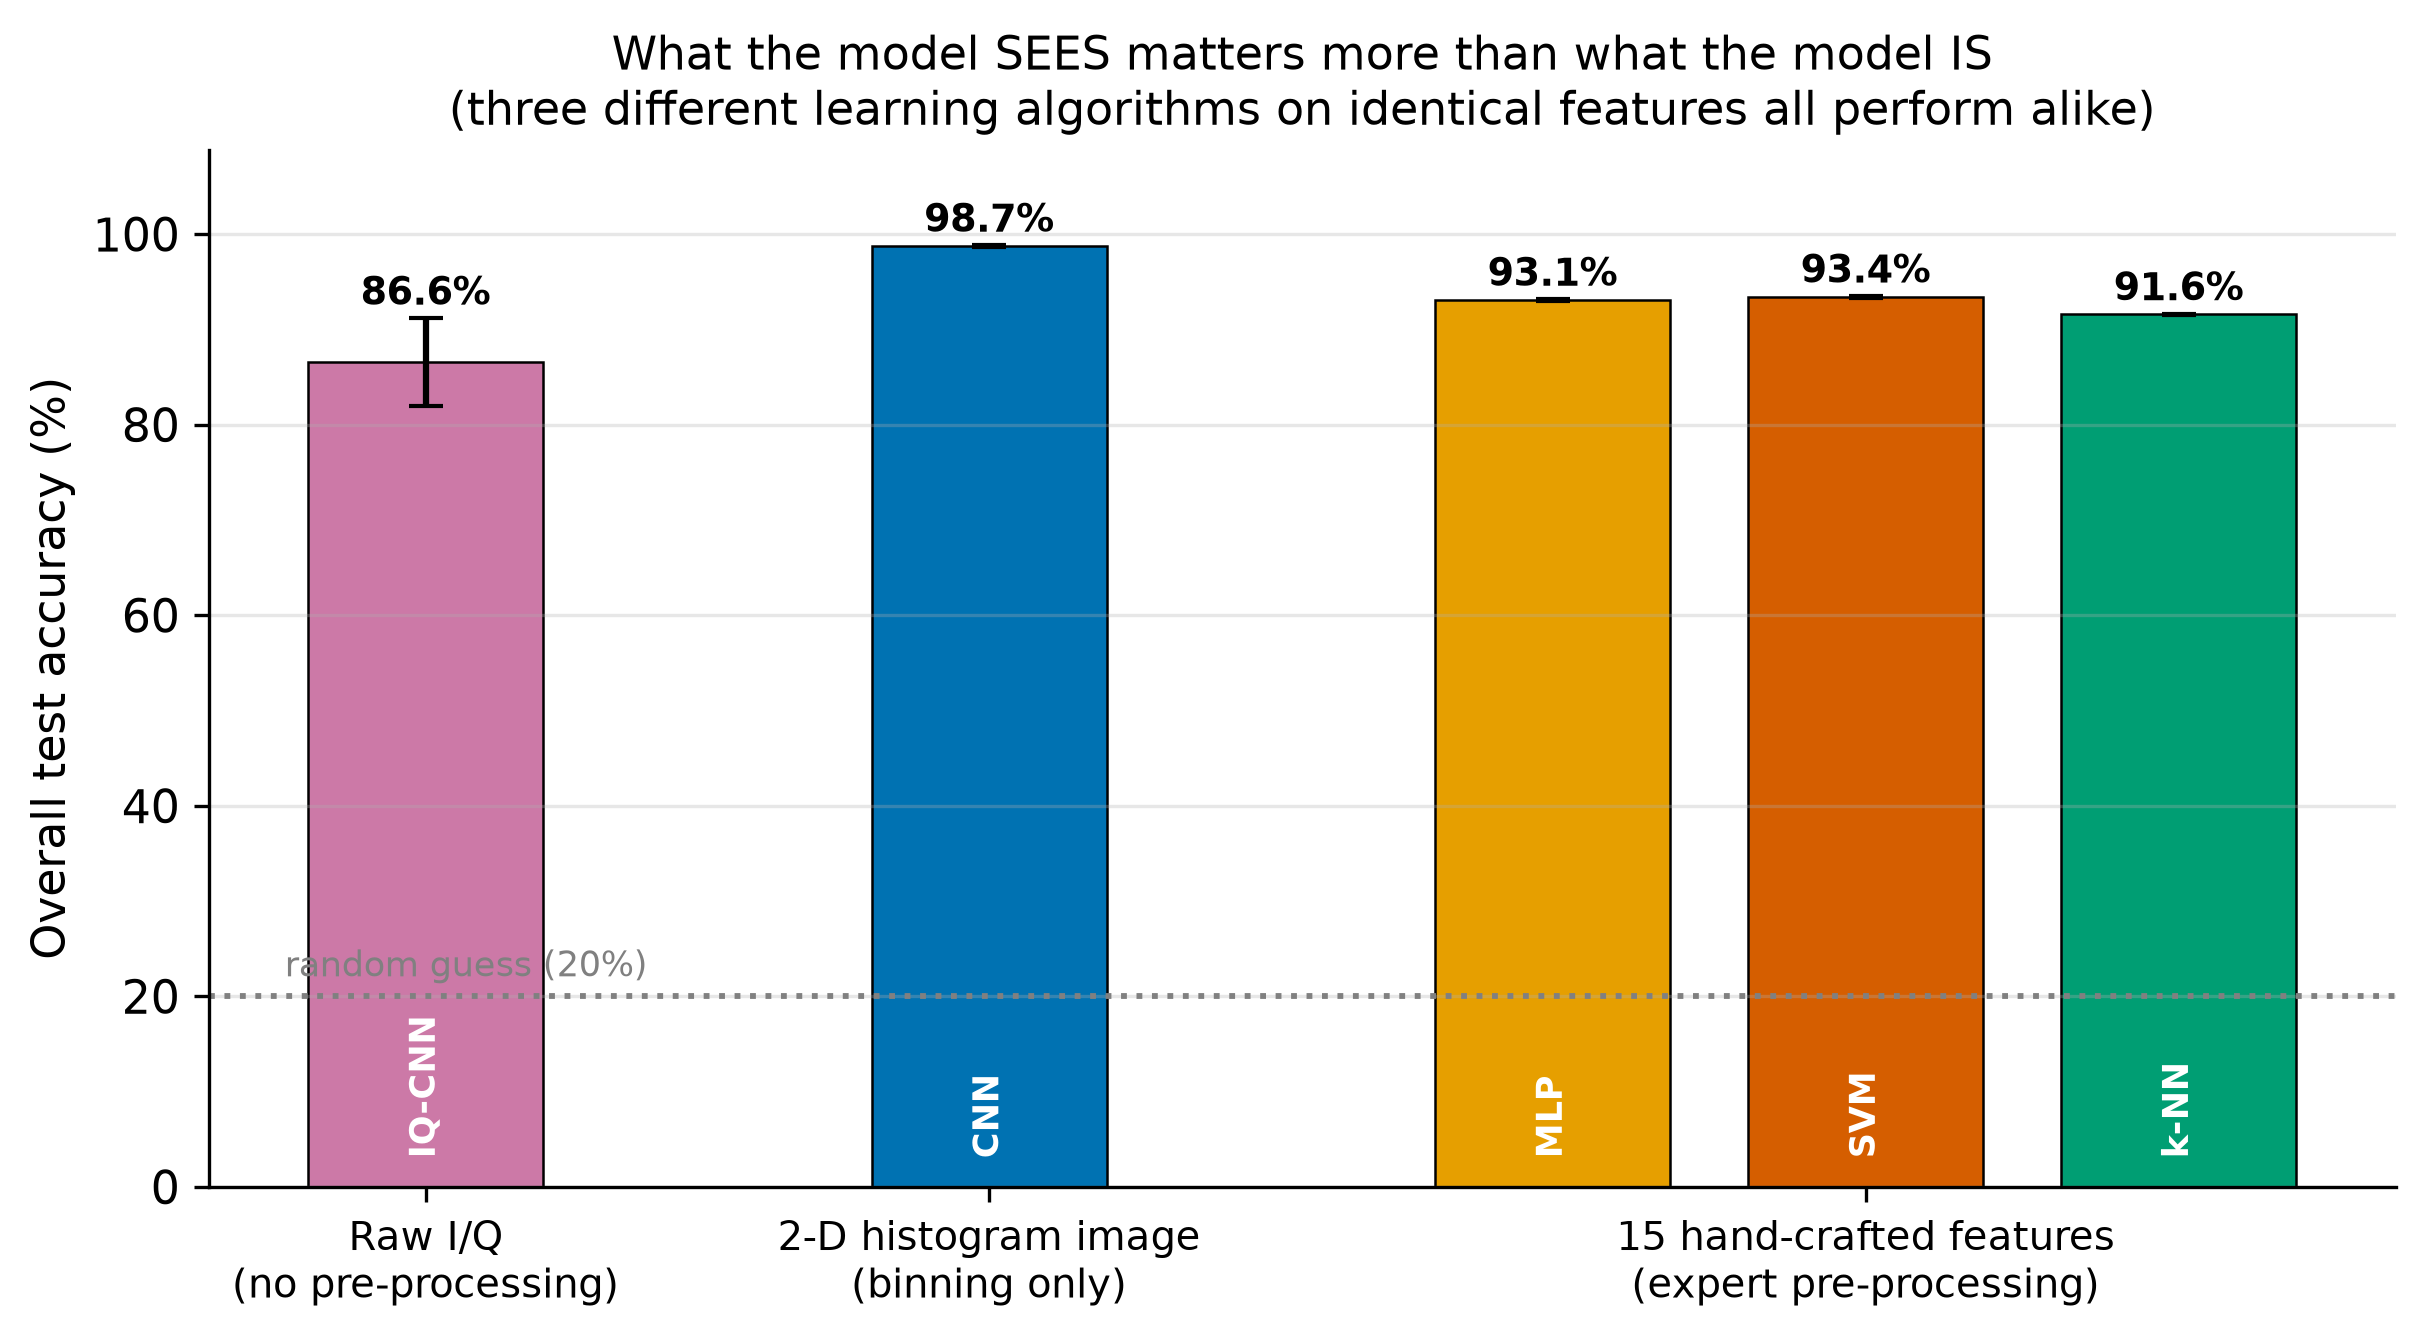
\includegraphics[width=\columnwidth]{fig2_representation.png}
\caption{Accuracy grouped by input representation. Three different learning
algorithms on identical hand-crafted features perform almost identically,
whereas changing the representation produces a large gain.}
\label{fig:representation}
\end{figure}

\subsection{Accuracy versus OSNR}

Fig.~\ref{fig:acc_osnr} shows accuracy against OSNR. All curves decrease with
decreasing OSNR, as they must: at low OSNR the constellation structure is
physically destroyed and no classifier can recover information the channel
has erased. The separation between methods is concentrated in the low-OSNR
regime: averaged over $5$--$10$~dB the CNN attains \CNNaccLow\% against
\SVMaccLow\% for the SVM, whereas over $20$--$25$~dB the CNN and all three
feature-based classifiers exceed \SVMaccHigh\%, becoming effectively
indistinguishable. The raw-I/Q model is the exception, plateauing at
\IQCNNaccHigh\% even at high OSNR.

Expressed as an OSNR margin --- the more meaningful quantity for a link
budget --- the CNN reaches $95\%$ accuracy at \CNNOSNRNinetyFive~dB against
\SVMOSNRNinetyFive~dB for the SVM, an advantage of \OSNRMargin~dB. A margin
of this size translates directly into additional reach or fewer inline
amplifiers.

\begin{figure}[t]
\centering
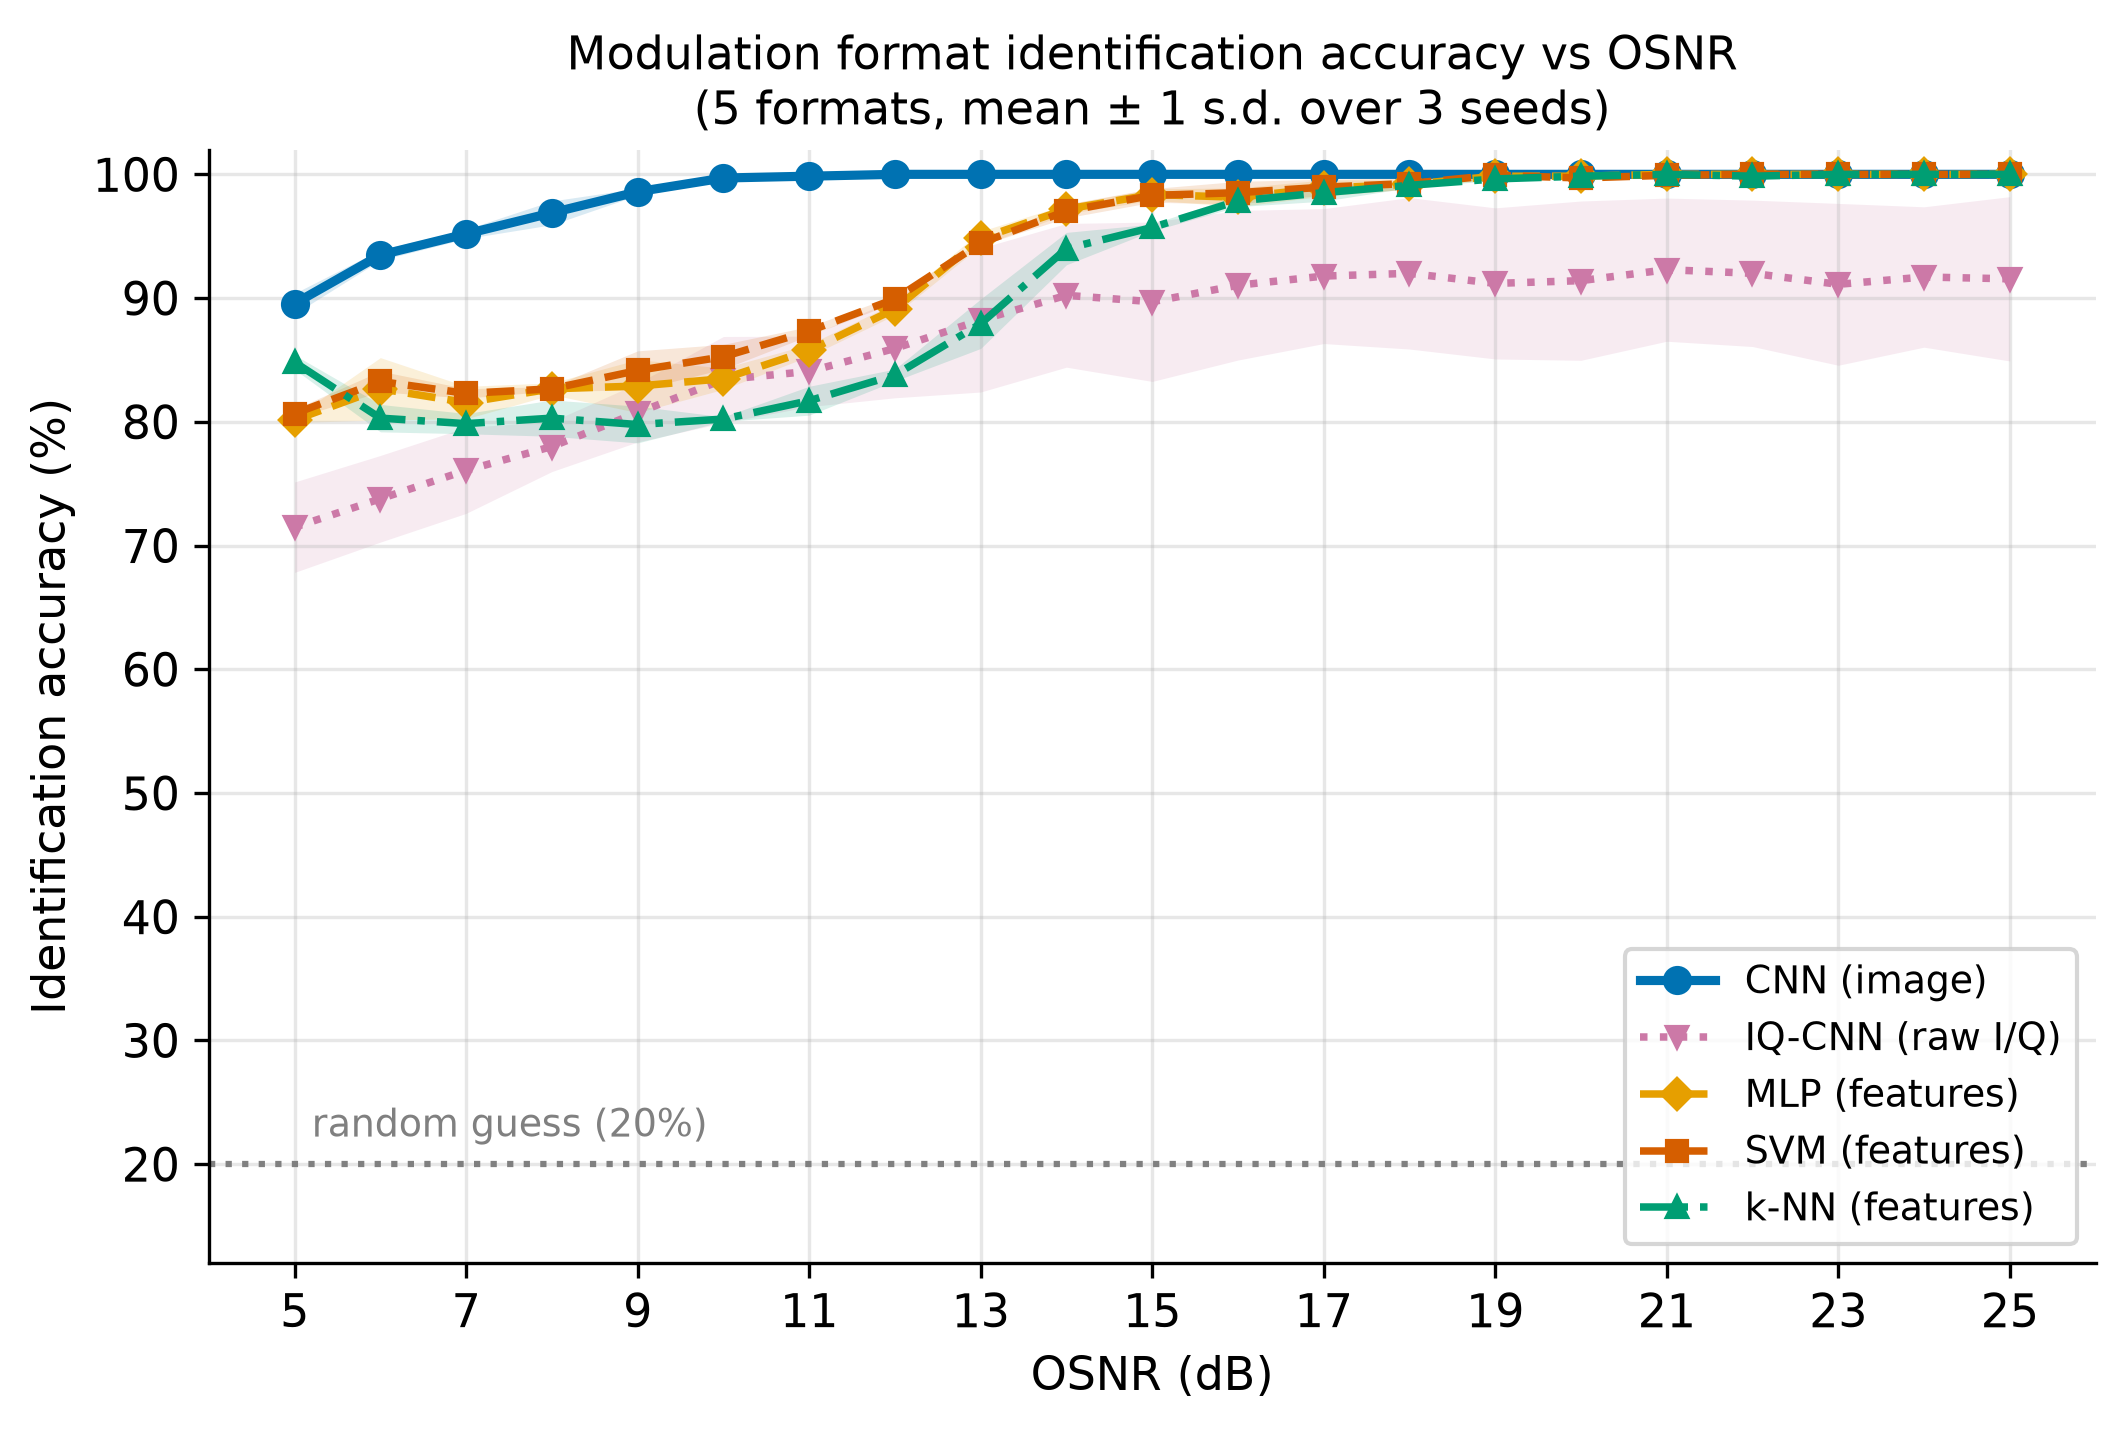
\includegraphics[width=\columnwidth]{fig1_accuracy_vs_osnr.png}
\caption{Identification accuracy versus OSNR. Shaded bands are $\pm$ one
standard deviation over \NumSeeds{} seeds. The dotted line is the
\ChanceLevel\% chance level for \NumFormats{} classes.}
\label{fig:acc_osnr}
\end{figure}

\subsection{Generalisation to unseen OSNR}

A model trained and tested on the same discrete OSNR grid might merely have
memorised the appearance of each level. To rule this out we retrain using
only even-valued OSNRs and test only on odd-valued ones, so that every test
condition is unseen. The CNN attains \CNNGenAcc$\pm$\CNNGenStd\%, a drop of
only \CNNGenDrop{} points relative to the matched case
(Fig.~\ref{fig:generalisation}). The model therefore interpolates across
noise levels rather than memorising them.

\begin{figure}[t]
\centering
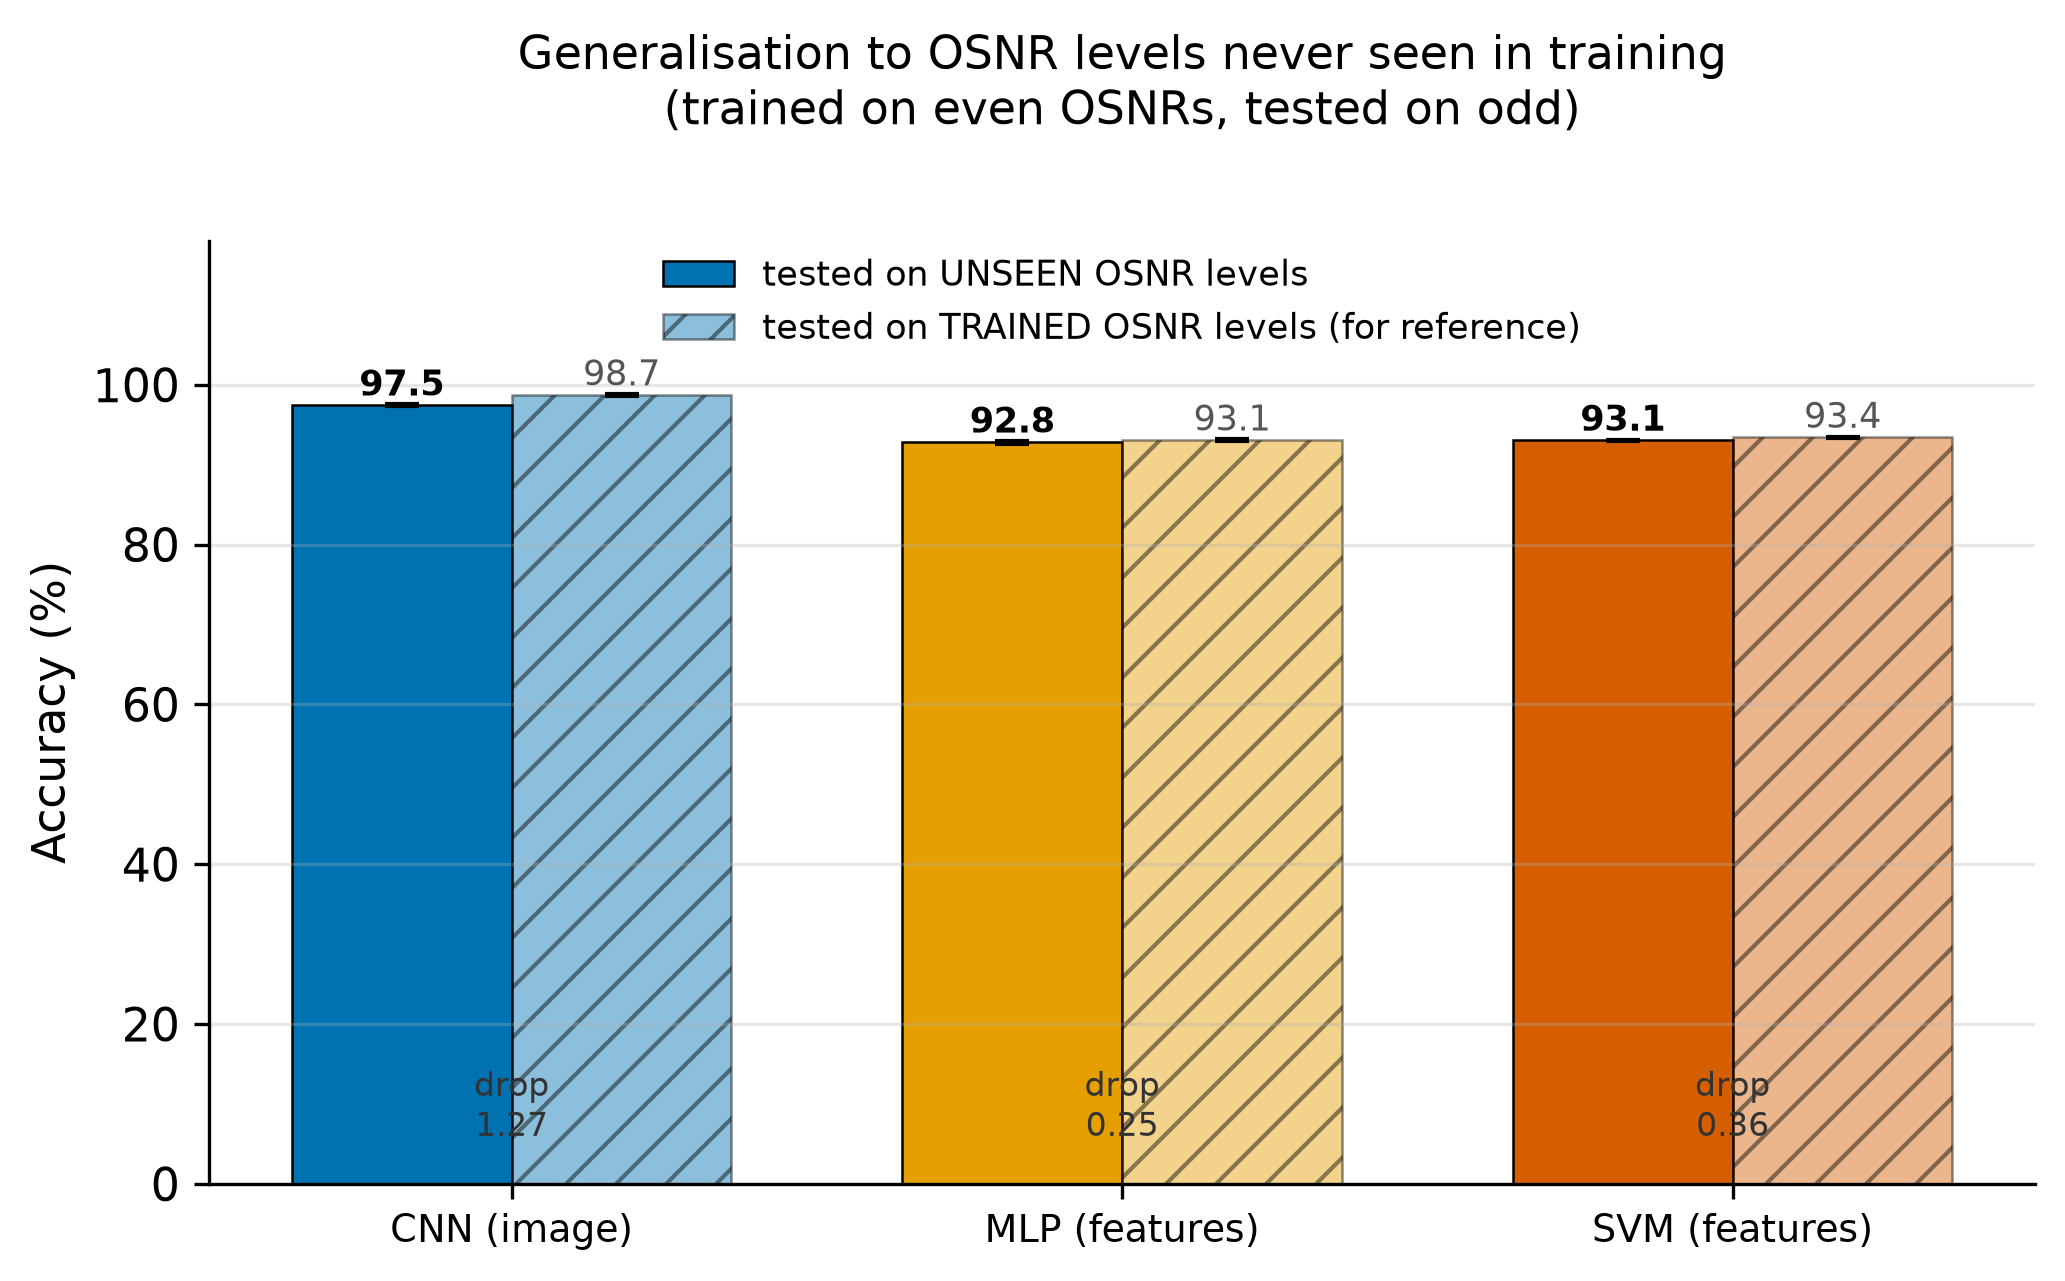
\includegraphics[width=\columnwidth]{fig9_generalisation.png}
\caption{Accuracy on OSNR levels withheld from training.}
\label{fig:generalisation}
\end{figure}

\subsection{Complexity and capture length}

An MFI block must eventually fit within a receiver's processing budget, so
accuracy alone is not the relevant figure of merit.
Fig.~\ref{fig:ablation} sweeps network depth and width.

Neither has much effect. Across all six
variants, accuracy spans only \AblSpread{} percentage points
(\AblMin--\AblMax\%), despite the largest configuration having
\AblParamRatio$\times$ more parameters and \AblMacRatio$\times$ more
arithmetic than the smallest. Holding width fixed at 16 channels, depth gives
\AblTwoBlockAcc\%, \AblThreeBlockAcc\% and \AblFourBlockAcc\% for two, three
and four blocks respectively: a monotonic but negligible gain. The smallest
configuration tested (\AblTinyParams{} parameters, \AblTinyMacs{}~MMAC per
inference) reaches \AblTinyAcc\%, against \AblBigAcc\% for the largest
(\AblBigParams{} parameters).

No optimum is claimed. This sweep used a single seed, and the non-monotonic
behaviour across widths indicates run-to-run variation of the same order as
the differences being measured. The conclusion supported by these data is
therefore the weaker one, that model capacity is not the binding constraint
within this family. This is consistent with the representation result of
Section~V-B, in that a small network suffices once the input is a density
image, and it indicates that an MFI block of well under $10^5$ parameters is a
realistic deployment target.

Fig.~\ref{fig:symbols} reports accuracy against capture length. Accuracy is
largely retained down to \SymEnough{} symbols (\SymEnoughAcc\%), compared
with \SymMaxAcc\% at \SymMax{} symbols. Short captures are therefore
sufficient, which relaxes the memory requirement of a practical monitor.

\begin{figure}[t]
\centering
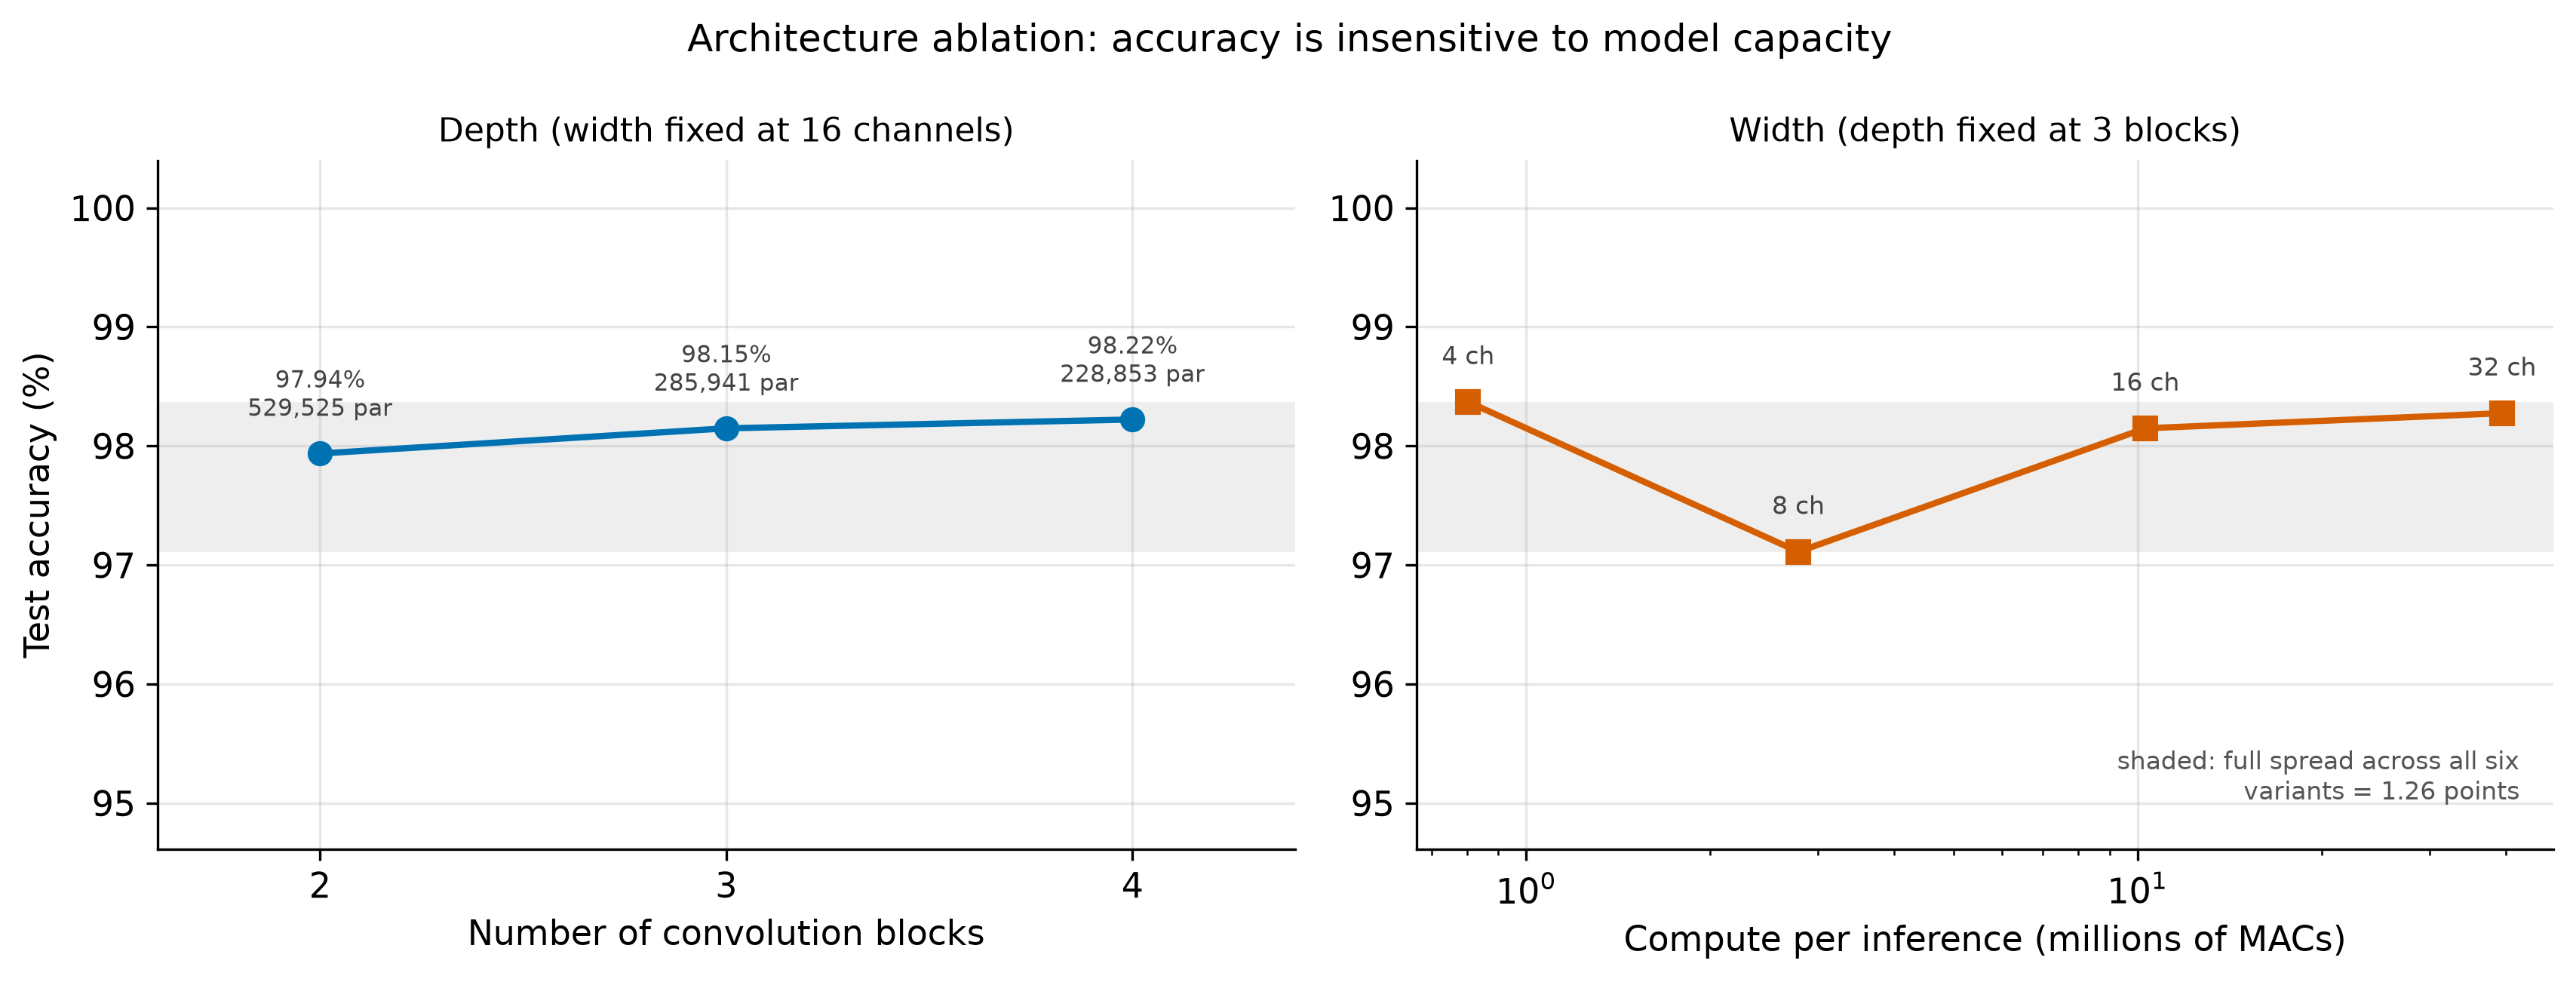
\includegraphics[width=\columnwidth]{fig6_ablation_pareto.png}
\caption{Architecture ablation: accuracy against depth and against compute.}
\label{fig:ablation}
\end{figure}

\begin{figure}[t]
\centering
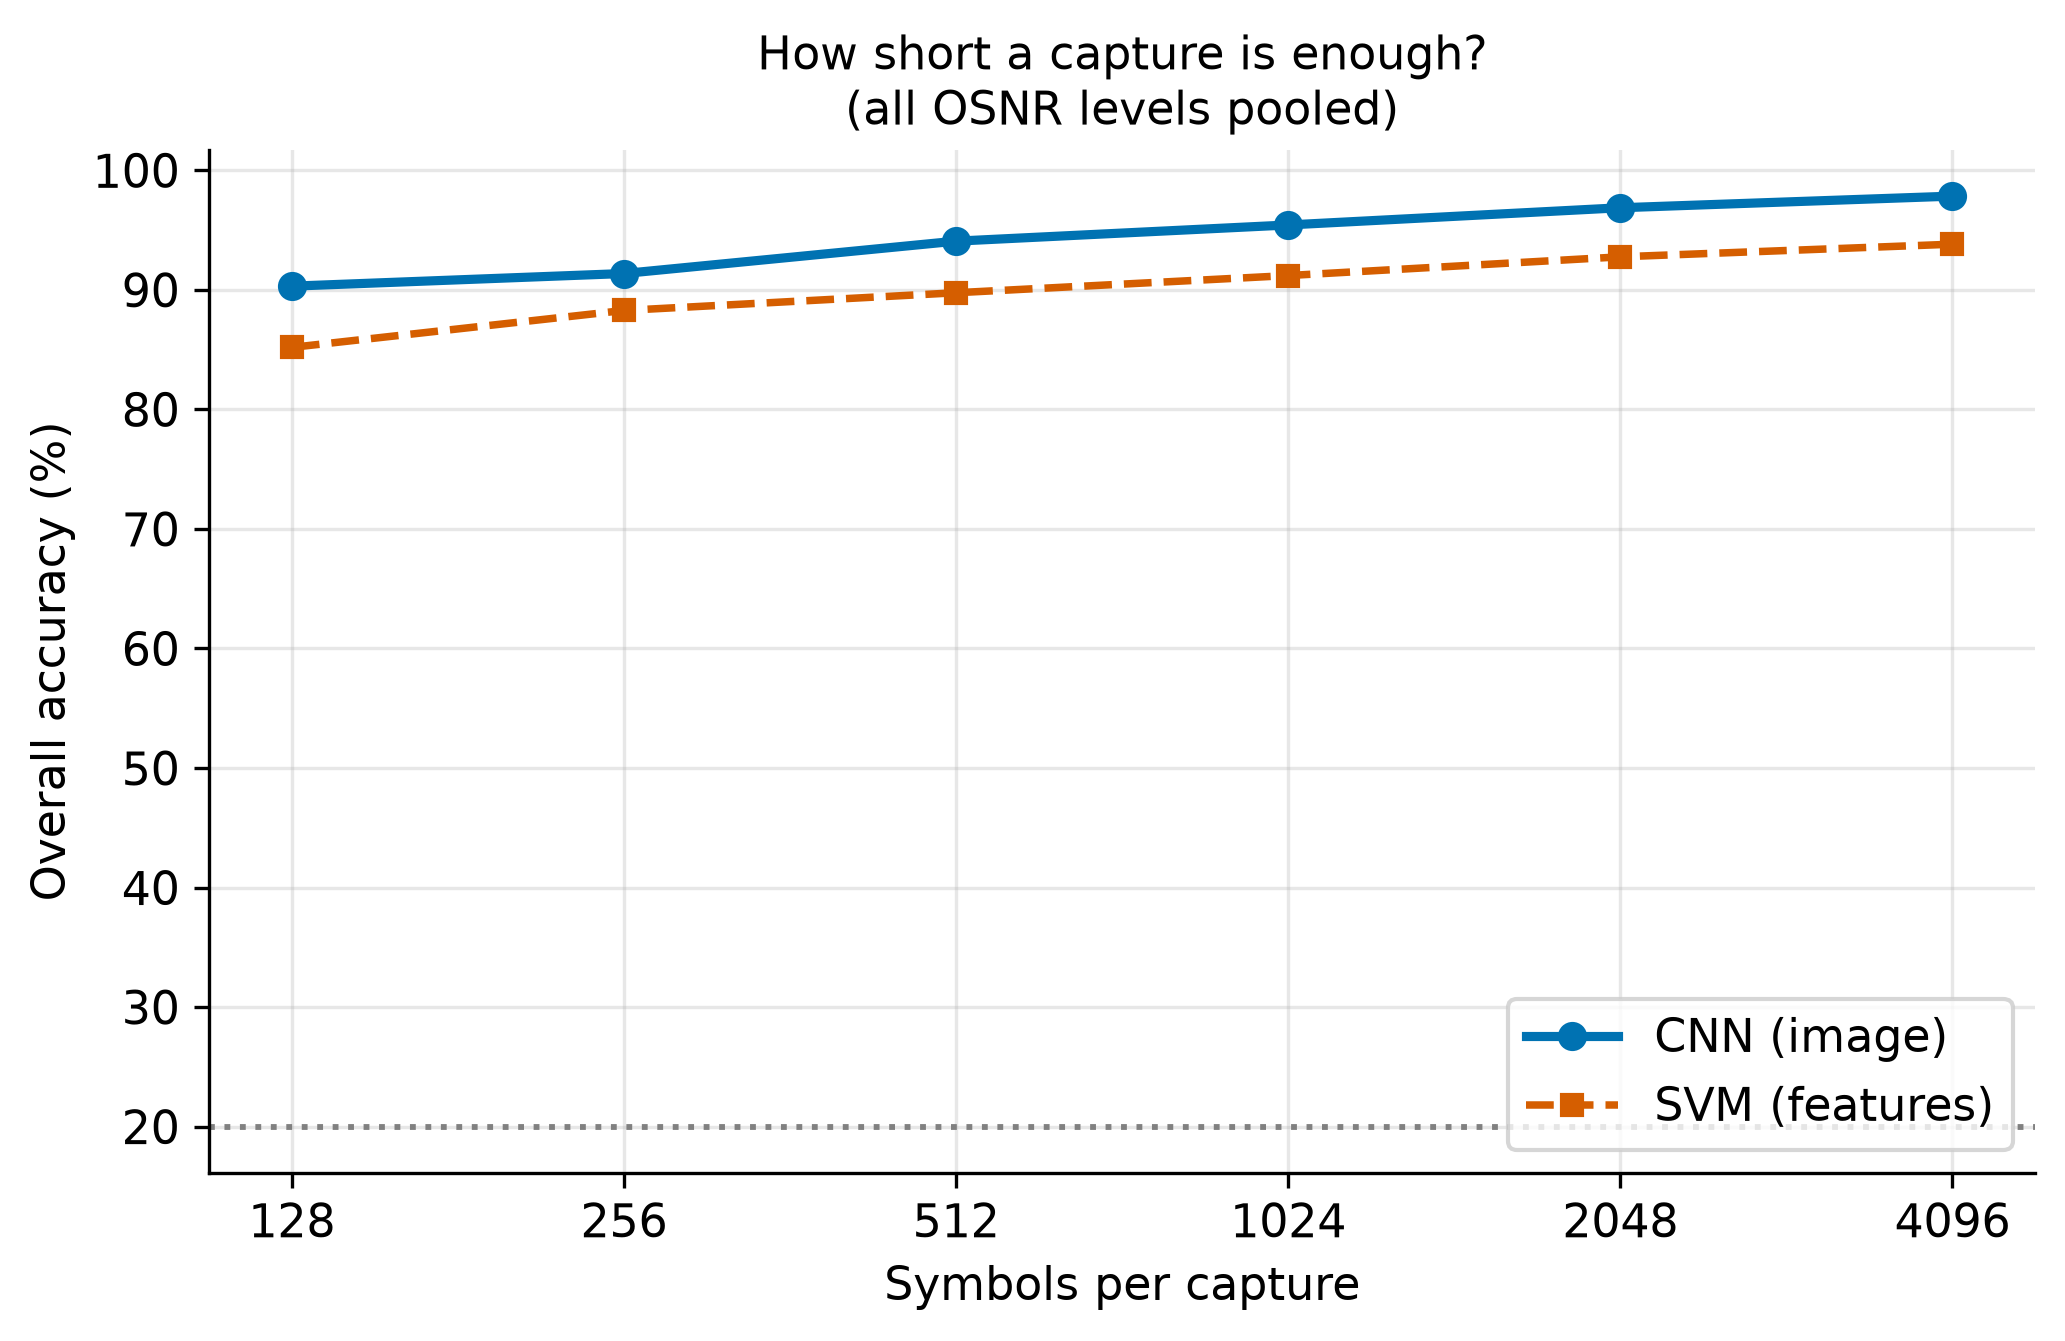
\includegraphics[width=\columnwidth]{fig7_symbols.png}
\caption{Accuracy against the number of symbols in the capture.}
\label{fig:symbols}
\end{figure}

\subsection{Robustness to unseen impairments}
\label{sec:robustness}

Finally we test transfer across channel conditions
(Fig.~\ref{fig:robustness}), training on one impairment profile and testing on
another. This is the setting that matters operationally: a model is trained on
a channel model, and then deployed on a link that may be worse than assumed.

The two representations behave very differently under mismatch. Trained on
the \textsc{ideal} AWGN-only channel and tested on \textsc{severe}, the CNN
falls from \RobIdealIdealCNN\% to \RobIdealSevereCNN\%, a drop of
\RobCNNDrop{} points. Under the same conditions the feature-based SVM falls
from \RobIdealIdealSVM\% to \RobIdealSevereSVM\%, a drop of \RobSVMDrop{}
points. With \NumFormats{} classes the chance level is \ChanceLevel\%, so the
feature-based classifier retains essentially no discriminative ability.

A plausible explanation is that higher-order cumulants are statistics of an
assumed signal model. I/Q imbalance, residual dispersion and phase error all
shift their values, so the decision boundaries learned in the
15-dimensional feature space no longer correspond to the same regions of
signal space. The CNN instead operates on the spatial structure of the density
image, where a distorted constellation continues to resemble its undistorted
form more closely than it resembles any other format, and degradation is
correspondingly gradual.

Training on the \textsc{realistic} profile recovers much of the loss for both
models (\RobRealSevereCNN\% and \RobRealSevereSVM\% respectively on
\textsc{severe}), confirming that the channel model used during training
materially determines deployed performance.

This result extends the contribution of Section~V-B. The advantage of the
density representation is not confined to matched conditions; it is larger
still under channel mismatch, which is the condition a simulation-trained
monitor encounters on deployment. It also suggests that matched-channel
accuracy, which is what the MFI literature generally reports, can substantially
overstate the performance available in practice.

\begin{figure}[t]
\centering
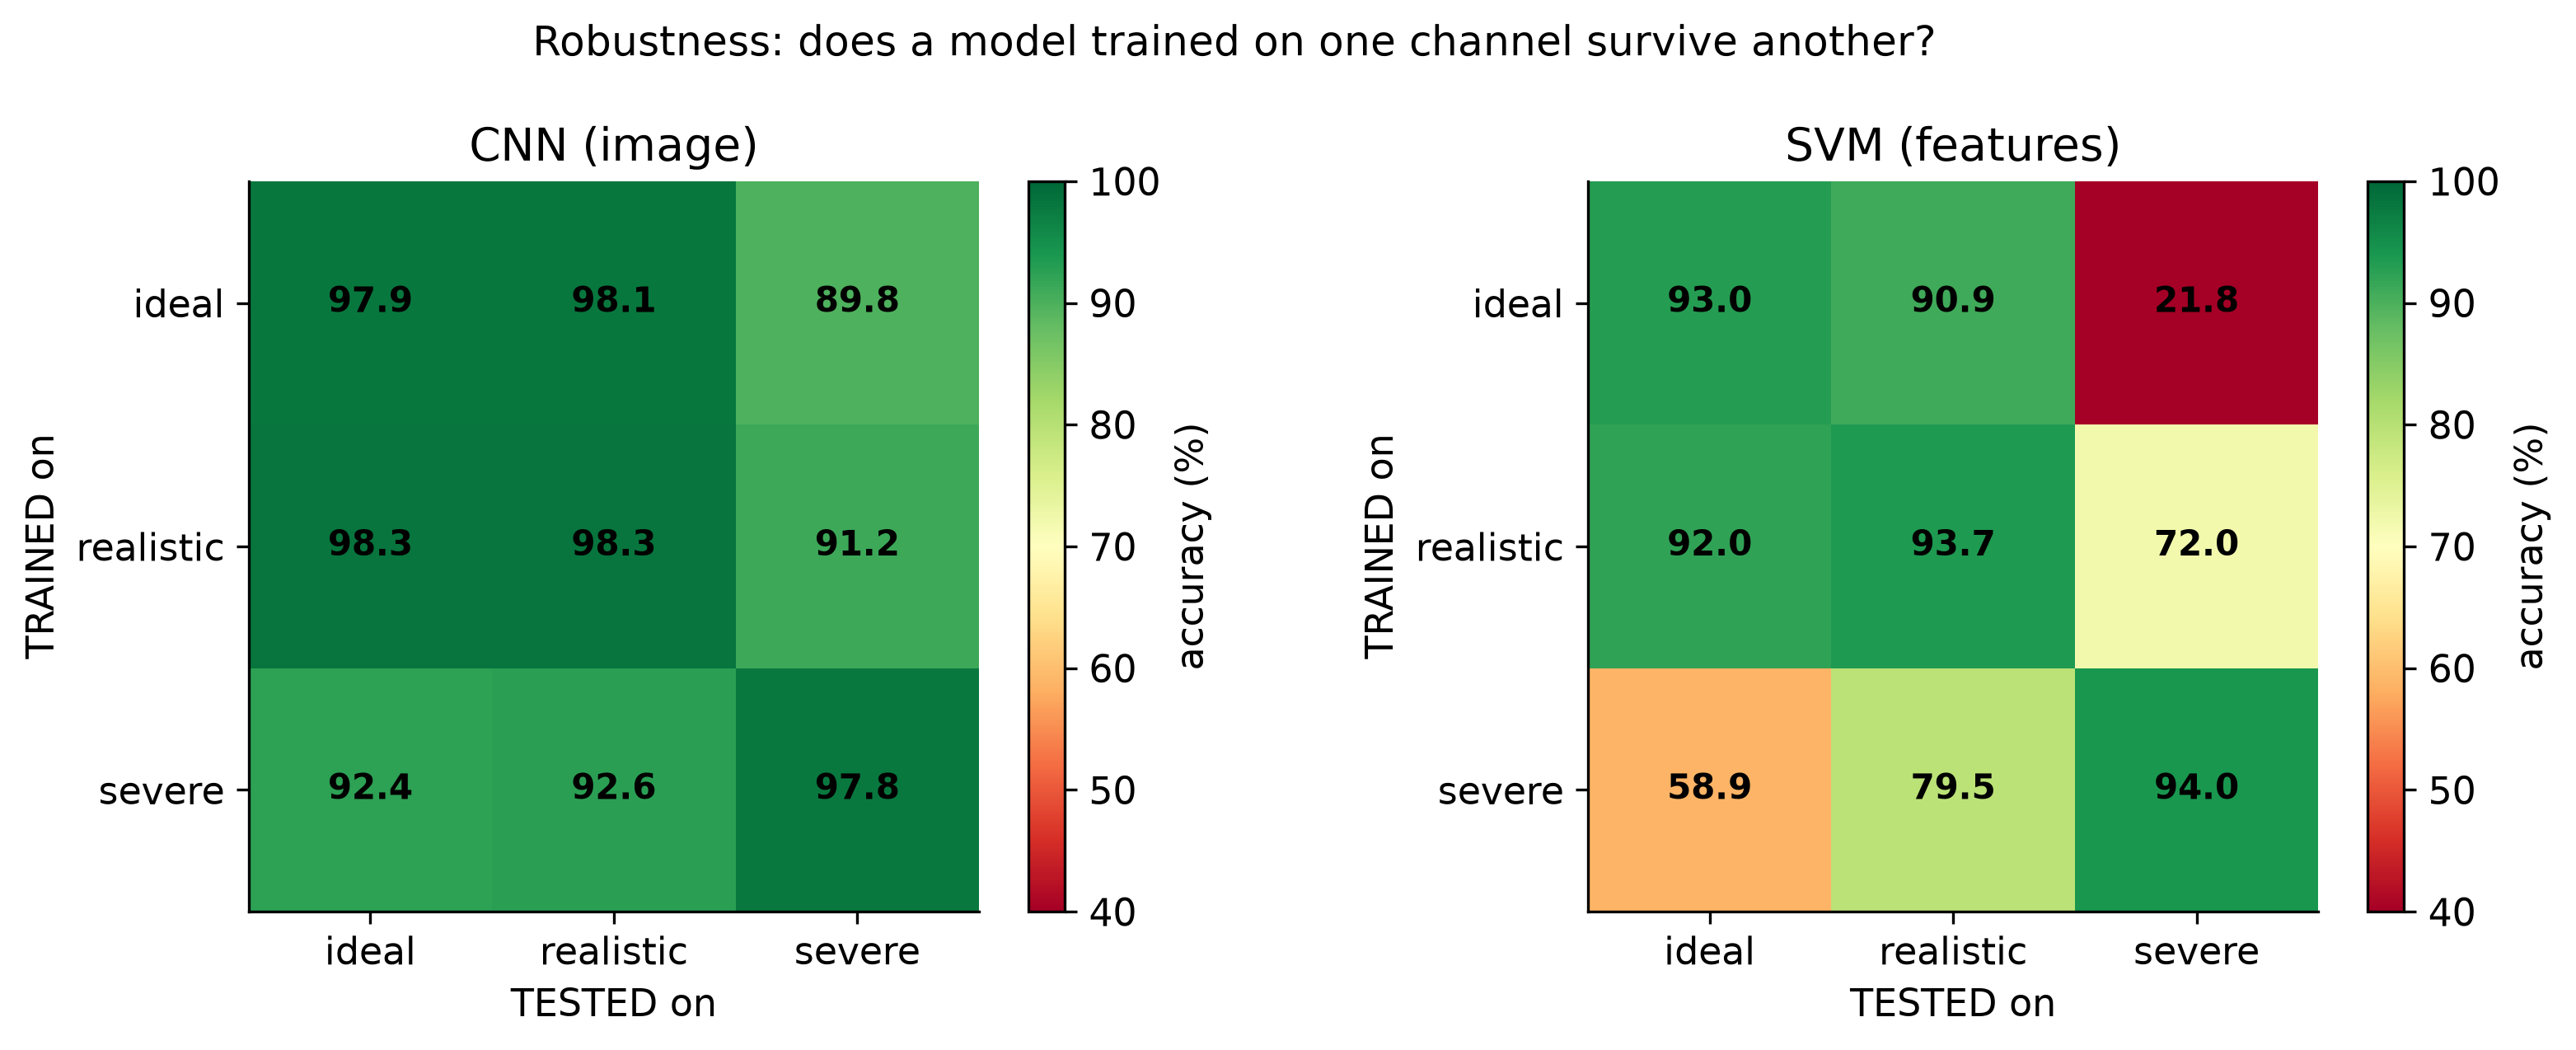
\includegraphics[width=\columnwidth]{fig8_robustness.png}
\caption{Cross-channel robustness. Rows: training profile. Columns: test
profile.}
\label{fig:robustness}
\end{figure}

\subsection{Does the model know when it is failing?}
\label{sec:confidence}

Section~\ref{sec:robustness} reports accuracy under channel mismatch, but
accuracy is visible only to the experimenter. A deployed monitor knows only
what it predicted and how confident it was. The operationally relevant
question is therefore whether the model's own confidence signals its failure,
and whether gating on that confidence keeps the monitor usable.

We take the maximum softmax probability as the confidence score, this being
the quantity a deployed system would threshold on, and use Platt scaling to
obtain the equivalent for the SVM. Models are trained on the \textsc{ideal}
channel and evaluated on \textsc{severe}.

Under matched conditions all three models are well calibrated, with mean
confidence within one percentage point of accuracy. Under mismatch they
diverge sharply (Fig.~\ref{fig:confidence}). The CNN falls to
\ConfCNNsevAcc\% accuracy while reporting \ConfCNNsevConf\% confidence, an
overconfidence of \ConfCNNsevOver{} points. The SVM falls to
\ConfSVMsevAcc\% --- barely above the \ChanceLevel\% chance level --- while
reporting \ConfSVMsevConf\% confidence, an overconfidence of
\ConfSVMsevOver{} points. It claims roughly twice the accuracy it achieves.

Confidence nonetheless remains informative in the ranking sense for both
models: the AUROC of confidence as a detector of the model's own errors is
\ConfCNNsevAuroc{} for the CNN and \ConfSVMsevAuroc{} for the SVM. Gating on
confidence should therefore restore reliability. The cost of doing so is where
the representations separate.

At a 90\% confidence gate on the \textsc{severe} channel, the CNN still
answers \ConfCNNCov90\% of inputs, at \ConfCNNAcc90\% accuracy on those it
answers. The SVM answers \ConfSVMCov90\% --- a coverage ratio of
approximately \CovRatio$\times$. The feature-based monitor can be made
accurate only by silencing it: at that operating point it responds to
approximately two inputs in every thousand. Under the milder
\textsc{realistic}-to-\textsc{severe} shift the same effect appears in
weaker form, with SVM coverage of \ConfSVMmodCov90\% at the same gate.

We therefore state the contribution of Section~V-B in a stronger form. The
input representation determines not only accuracy under matched conditions,
but whether a confidence-gated monitor remains \emph{operational} under
mismatch at all. To our knowledge this interaction between input
representation and failure self-detectability has not previously been
reported; uncertainty quantification for modulation classification has been
studied for a single representation~\cite{yang2025uq}, and representation
comparison has been studied for accuracy alone~\cite{ge2021accuracy}.

\begin{figure}[t]
\centering
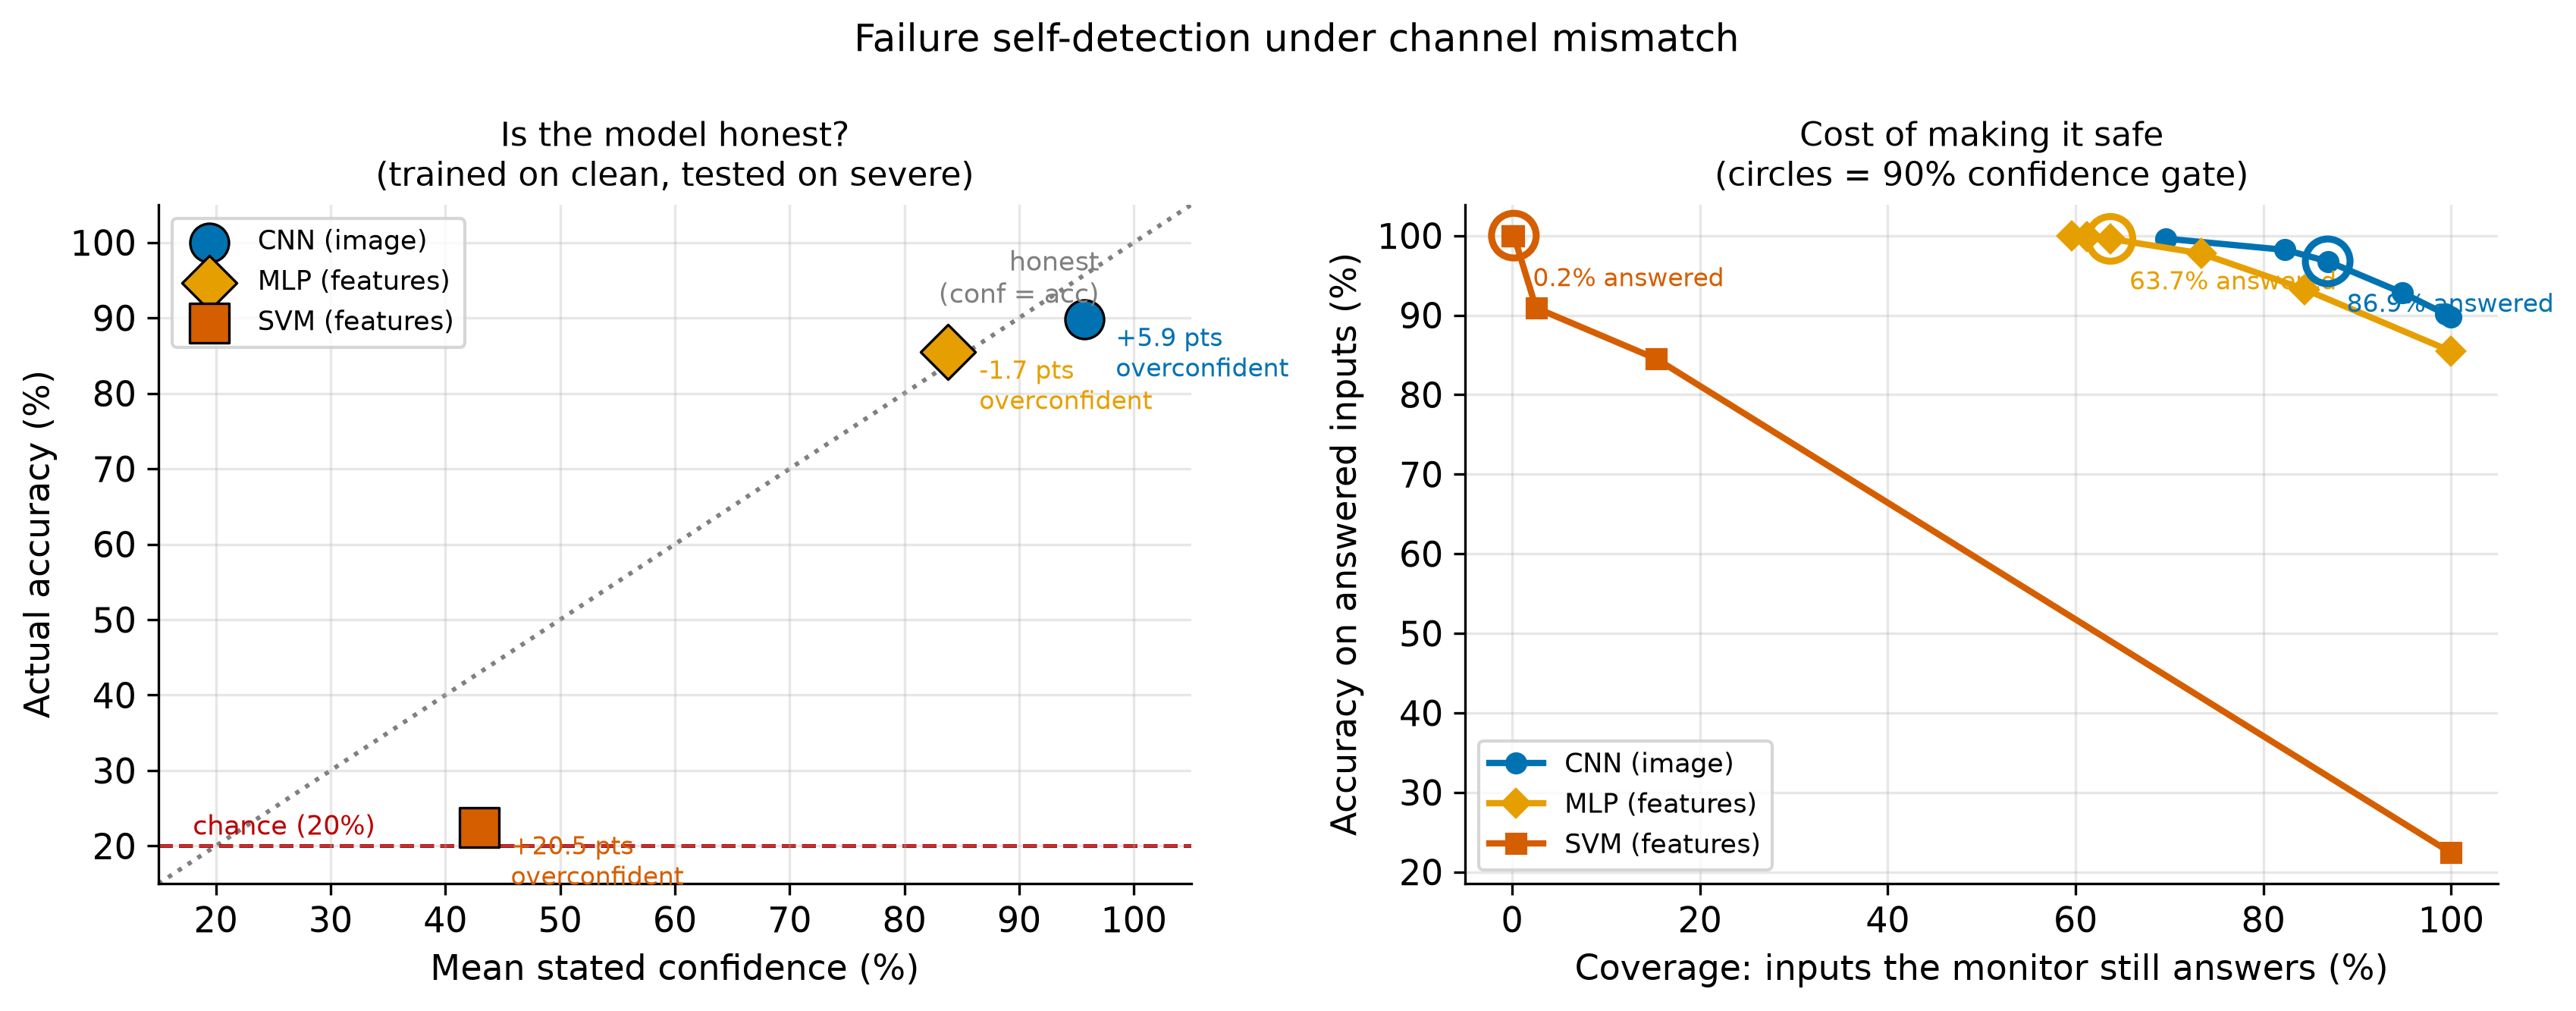
\includegraphics[width=\columnwidth]{fig10_confidence.png}
\caption{Failure self-detection under channel mismatch. Left: stated
confidence against actual accuracy on the unseen \textsc{severe} channel;
the dotted diagonal marks an honest model. Right: the accuracy--coverage
trade-off under confidence gating, with circles marking the 90\% gate.}
\label{fig:confidence}
\end{figure}

\subsection{Impairment tolerance budget}
\label{sec:tolerance}

Sections~\ref{sec:robustness} and~\ref{sec:confidence} compare discrete
channel profiles, which establishes that mismatch is harmful but not how much
mismatch is affordable. We therefore vary one impairment at a time, holding
the remaining four at their training values, and record accuracy as that
parameter moves away from the value the model was trained on
(Fig.~\ref{fig:tolerance}). Models are trained once on the \textsc{realistic}
channel; no retraining is performed.

Table~\ref{tab:tolerance} reports the largest tested deviation at which each
model still achieves 90\% accuracy. Three observations follow.

First, the two representations do not fail through the same mechanism. The
feature-based classifier is highly sensitive to the two impairments that
distort constellation \emph{geometry}: accuracy falls from \TolSVMgainLo\% to
\TolSVMgainHi\% as I/Q gain imbalance increases from 0.3~dB to 2.5~dB, and
from \TolSVMskewLo\% to \TolSVMskewHi\% as I/Q phase skew increases from
$2^\circ$ to $14^\circ$ --- the \ChanceLevel\% chance level in both cases. The
CNN retains \TolCNNgainHi\% and \TolCNNskewHi\% respectively at the same
extremes. This is consistent with the mechanism proposed in
Section~\ref{sec:robustness}: cumulants are moments computed under an
implicit assumption of balanced quadratures, so a geometric skew corrupts them
directly, whereas a skewed constellation image remains recognisable as a
skewed version of the correct constellation.

Second, and contrary to the pattern elsewhere in this paper, the feature-based
classifier is \emph{more} tolerant of residual chromatic dispersion: at
150~ps/nm it retains \TolSVMcdHi\% against \TolCNNcdHi\% for the CNN. This is
also
consistent with the same mechanism. Dispersion-induced inter-symbol
interference broadens the symbol cloud in a manner closer to added noise than
to geometric distortion, and higher-order cumulants are specifically
constructed so that Gaussian contributions cancel. We report this because it
qualifies the paper's central claim: the density representation is not
uniformly superior, and its advantage is specific to distortions that preserve
gross constellation structure while altering its geometry.

Third, laser linewidth is essentially irrelevant to both models over the
entire range tested, up to 2~MHz, because block-average carrier phase recovery
removes it. Residual frequency offset affects both models identically, with a
sharp common failure between 50~MHz and 100~MHz.

The practical reading is that a designer intending to train an MFI monitor on
a simulated channel must characterise I/Q imbalance far more accurately than
laser linewidth, and that the required accuracy depends on the representation:
approximately $4\times$ tighter for a cumulant-based monitor than for an
image-based one.

\begin{table}[t]
\caption{Impairment tolerance budget: largest tested deviation still meeting
90\% accuracy. Arrows mark the more tolerant representation.}
\label{tab:tolerance}
\centering
\begin{tabular}{lrrl}
\toprule
Impairment & CNN & SVM & \\
\midrule
Laser linewidth      & $>$\BudgetCNNLw{} kHz & $>$\BudgetSVMLw{} kHz & equal \\
Frequency offset     & \BudgetCNNFoff{} MHz & \BudgetSVMFoff{} MHz & equal \\
I/Q gain imbalance   & $>$\BudgetCNNGain{} dB & \BudgetSVMGain{} dB & CNN $\geq4\times$ \\
I/Q phase skew       & $>$\BudgetCNNSkew$^\circ$ & \BudgetSVMSkew$^\circ$ & CNN $\geq3.5\times$ \\
Residual dispersion  & \BudgetCNNCD{} ps/nm & \BudgetSVMCD{} ps/nm & SVM $1.8\times$ \\
\bottomrule
\end{tabular}
\end{table}

\begin{figure*}[t]
\centering
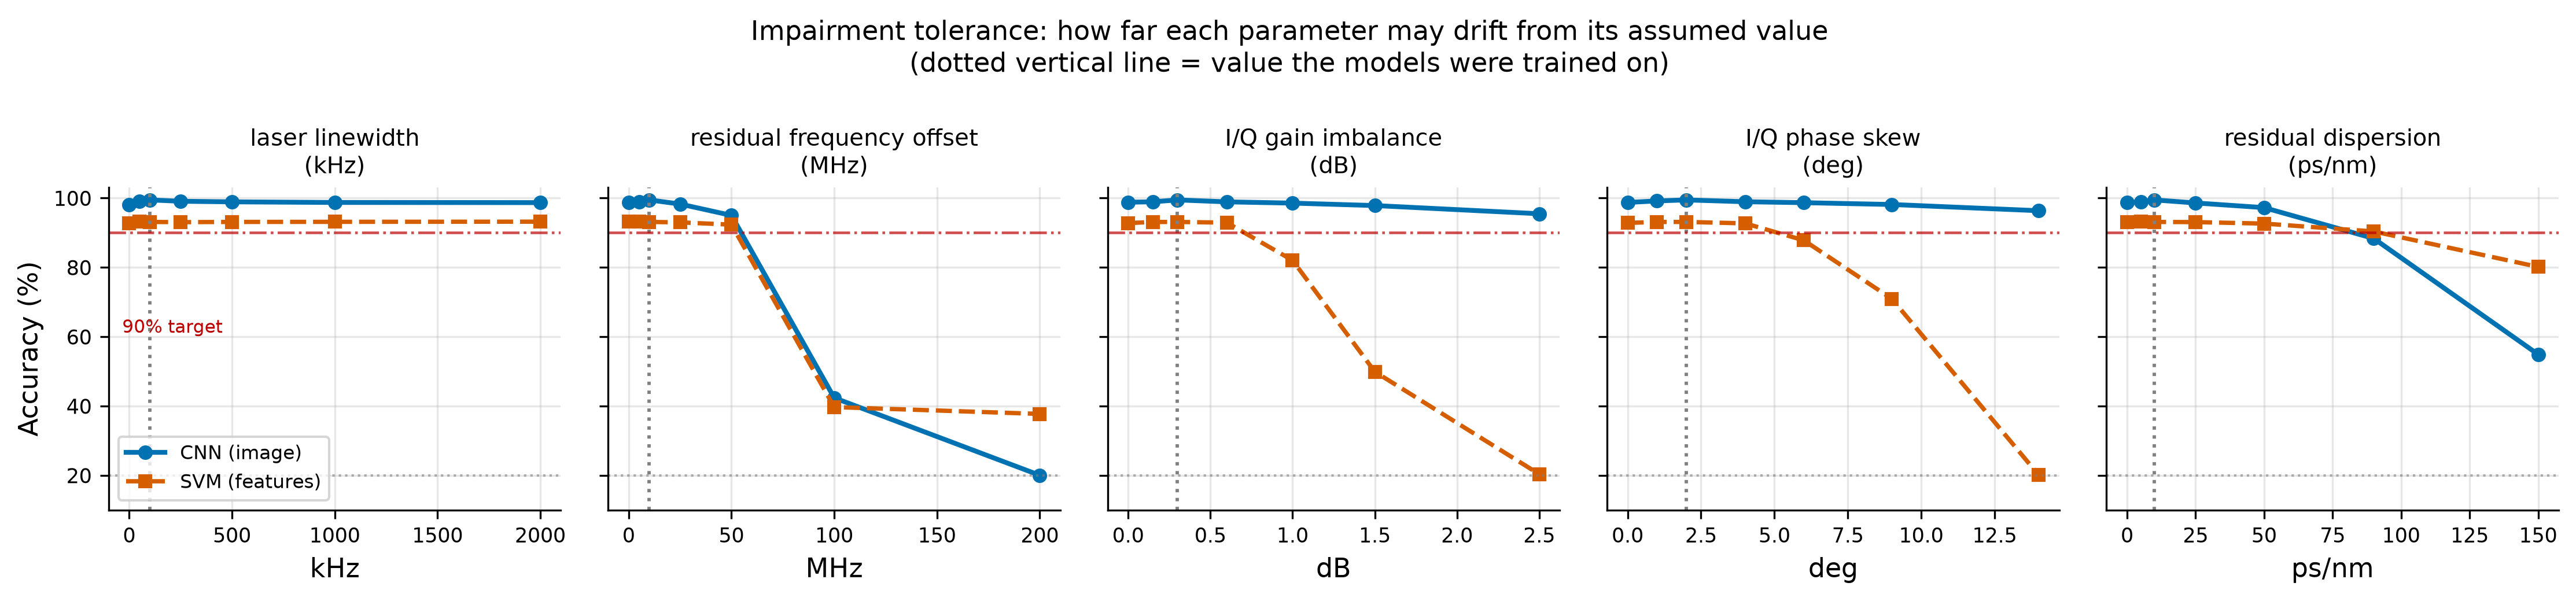
\includegraphics[width=\textwidth]{fig11_tolerance.png}
\caption{Impairment tolerance. Each panel sweeps one impairment while the
others are held at their training values. The dotted vertical line marks the
trained value; the dash-dotted horizontal line marks a 90\% accuracy target.}
\label{fig:tolerance}
\end{figure*}

%=============================================================================
\section{Discussion}

The results suggest a practical design rule for MFI: invest in the input
representation before investing in model capacity. A modest CNN on a density
image outperforms both a deeper-in-spirit model on raw samples and three
different learners on expert features, and the ablation shows that most of
its capacity is not needed.

A likely mechanism is the following. The discriminative information in MFI is
the distribution of received symbols in the complex plane. A two-dimensional
histogram is a direct non-parametric estimate of that distribution, so the CNN
begins from a near-sufficient statistic and need only classify its shape.
Cumulants are also statistics of the same distribution, but constitute a lossy
15-dimensional projection of it chosen in advance. The raw sample stream
retains all of the information, but presents it in a time-indexed form from
which the density must be re-estimated by the network.

\textbf{Limitations.} The evaluation is simulation-based; no experimental
captures are used. We model single-polarisation transmission, a single symbol
rate, and a linear channel --- fibre nonlinearity, polarisation-mode
dispersion and polarisation multiplexing are not included. The RBF-SVM is
trained on a capped subsample for tractability. Extending the study to
experimental data, to polarisation-multiplexed transmission and to joint
format-and-OSNR estimation are natural next steps.

%=============================================================================
\section{Conclusion}

We separated the contributions of model and representation in
machine-learning modulation format identification. On a common benchmark of
\NumImages{} captures spanning \NumFormats{} formats and a realistically
impaired channel, varying the learning algorithm over identical inputs
changed accuracy by \FeatSpread{} percentage points, while varying the input
representation changed it by \RepGain{} points, a ratio of approximately
\RepRatio. A trained multilayer perceptron on hand-crafted features did not
outperform a kernel machine on the same features, which indicates that model
capacity was not the limiting factor.

A compact CNN on constellation density images achieved \CNNacc\% overall, an
OSNR margin of \OSNRMargin~dB over the best feature-based classifier, and
\CNNGenAcc\% on OSNR values withheld from training. Its largest advantage
occurred under channel mismatch, where the feature-based classifier fell to
the \ChanceLevel\% chance level while the CNN retained
\RobIdealSevereCNN\%.

We conclude that the input representation, rather than model capacity, is the
dominant design variable for this task; that the benefit is one of robustness
as much as accuracy; and that the channel model used during training
substantially determines whether either transfers.

%=============================================================================
\section*{Reproducibility}

All source code, the data-generation simulator, trained model weights and the
scripts that produce every figure and number in this paper are available at
\url{https://github.com/techi101/optical-mfi-representation}. All experiments
run on a single CPU; no GPU is required.
Random seeds are fixed and an automated verification script re-derives the
reported accuracies from the saved model weights.

%=============================================================================
\begin{thebibliography}{00}

\bibitem{khan2019perspective}
F.~N. Khan, Q.~Fan, C.~Lu, and A.~P.~T. Lau, ``An optical communication's
perspective on machine learning and its applications,'' \emph{J. Lightw.
Technol.}, vol.~37, no.~2, pp.~493--516, 2019.

\bibitem{swami2000cumulants}
A.~Swami and B.~M. Sadler, ``Hierarchical digital modulation classification
using cumulants,'' \emph{IEEE Trans. Commun.}, vol.~48, no.~3, pp.~416--429,
2000.

\bibitem{dobre2007survey}
O.~A. Dobre, A.~Abdi, Y.~Bar-Ness, and W.~Su, ``Survey of automatic
modulation classification techniques: classical approaches and new trends,''
\emph{IET Commun.}, vol.~1, no.~2, pp.~137--156, 2007.

\bibitem{wang2017analyzer}
D.~Wang \emph{et al.}, ``Intelligent constellation diagram analyzer using
convolutional neural network-based deep learning,'' \emph{Opt. Express},
vol.~25, no.~15, pp.~17150--17166, 2017.

\bibitem{khan2016deep}
F.~N. Khan, K.~Zhong, W.~H. Al-Arashi, C.~Yu, C.~Lu, and A.~P.~T. Lau,
``Modulation format identification in coherent receivers using deep machine
learning,'' \emph{IEEE Photon. Technol. Lett.}, vol.~28, no.~17,
pp.~1886--1889, 2016.

\bibitem{oshea2016radio}
T.~J. O'Shea, J.~Corgan, and T.~C. Clancy, ``Convolutional radio modulation
recognition networks,'' in \emph{Engineering Applications of Neural Networks
(EANN 2016)}, Commun. Comput. Inf. Sci., vol.~629. Cham, Switzerland:
Springer, 2016, pp.~213--226.

\bibitem{ge2021accuracy}
Z.~Ge, H.~Jiang, Y.~Guo, and J.~Zhou, ``Accuracy analysis of feature-based
automatic modulation classification via deep neural network,''
\emph{Sensors}, vol.~21, no.~24, 8252, 2021.

\bibitem{huang2022svm}
Z.~Huang, Q.~Zhang, X.~Xin, H.~Yao, R.~Gao, J.~Jiang, F.~Tian, B.~Liu,
F.~Wang, and Q.~Tian, ``Modulation format identification based on signal
constellation diagrams and support vector machine,'' \emph{Photonics},
vol.~9, no.~12, art.~927, 2022.

\bibitem{amcsurvey2025}
X.~Tian \emph{et al.}, ``A survey on deep learning enabled automatic
modulation classification methods: data representations, model structures,
and regularization techniques,'' \emph{Signal Processing}, 2025.

\bibitem{yang2025uq}
H.~Yang and R.~Sahay, ``An uncertainty quantification framework for deep
learning-based automatic modulation classification,'' \emph{arXiv preprint
arXiv:2503.04142}, 2025.

\end{thebibliography}

\end{document}
